\documentclass[a4paper]{article}

\usepackage[utf8]{inputenc}
\usepackage[T1]{fontenc,url}
\usepackage{cite}
\usepackage{hyperref}
\usepackage{amsmath, amssymb}
\usepackage{tikz}
\usepackage{graphicx}
\usepackage{parskip}
\usepackage{lmodern}
\usepackage{algorithm}
\usepackage{algpseudocode}
\usepackage{epigraph}
\usepackage{listings}
\usepackage{float}
\usepackage{amsthm}
\usepackage{changepage}
\usepackage{listings}



\newcommand{\dydx}{\frac{\partial\psi}{\partial x}}
\newcommand{\dydy}{\frac{\partial\psi}{\partial y}}
\newcommand{\dyydxx}{\frac{\partial^2\psi}{\partial x^2}}
\newcommand{\dyydyy}{\frac{\partial^2\psi}{\partial y^2}}
\newcommand{\dydt}{\frac{\partial\zeta}{\partial t}}
\newcommand{\dyydtt}{\frac{\partial^2\zeta}{\partial t^2}}
\newcommand{\Ixyt}{|_{x,y}^{t}}
\newcommand{\IIxyt}{\Bigr|_{x,y}^{t}}
\newcommand{\Ixytp}{|_{x,y}^{t\pm\Delta t}}
\newcommand{\Ixytm}{|_{x,y}^{t-\Delta t}}
\newcommand{\Ixpyt}{|_{x\pm\Delta x,y}^{t}}
\newcommand{\Ixmyt}{|_{x-\Delta x,y}^{t}}
\newcommand{\Ixypt}{|_{x,y\pm\Delta y}^{t}}
\newcommand{\Ixymt}{|_{x,y-\Delta y}^{t}}
\newcommand{\Ijkn}{|_{j,k}^{n}}
\newcommand{\Ijknp}{|_{j,k}^{n+1}}
\newcommand{\IIjknp}{\Bigr|_{j,k}^{n+1}}
\newcommand{\Ijpkn}{|_{j+1,k}^{n}}
\newcommand{\Ijmkn}{|_{j-1,k}^{n}}

\begin{document}
\title{FYS4150 -- Project 5}
\author{Joachim Falck Brodin,
        Fredrik Jaibeer Mahal Nordeng,\\ 
        and Endrias Getachew Asgedom}

\maketitle
\begin{abstract}
We revisit the results of the article by Katarzyna Sznajd-Weron and Józef Sznajd \cite{opinion}. The topic is numerical simulations on a variation of the 1D Ising model, with modified rules, as a model for opinion evaluation in a closed community. The model allows for a 1D array (vector) of individuals with each one holding one of two opinions (spin \textit{up}, or spin \textit{down}). Through Monte Carlo (MC) cycles the vector is gradually transformed and the spins self organize into clusters of either one of the opposing opinions or of alternating spins of each opinion. The system inevitably leads to the whole system being fully fixed in one of the three configurations, with probabilities of 25\% for each of the opinions and 50\% for the state of alternating opinions. We confirm a power law, $P(\tau)\sim \tau^{-3/2}$ , for the probability distribution of the decision time, $\tau$, for single individuals. We also find similar results with the introduction of a probability, $p$, that the drawn spins disobey the rules, leading to another function describing the probability distribution of the decision time. In addition to confirming the findings from \cite{opinion}, we investigate the mean cluster size for a very large system as a function of MC-cycles. The cluster mean size fluctuates locally over the MC-cycles, but overall the system organizes into fewer clusters, and thus, larger mean cluster sizes.



%Their:A simple Ising spin model which can describe a mechanism of
%making a decision in a closed community is proposed. It is shown via standard
%Monte Carlo simulations that very simple rules lead to rather complicated
%dynamics and to a power law in the decision time distribution. It is found
%that a closed community has to evolve either to a dictatorship or a stalemate
%state (inability to take any common decision). A common decision can be
%taken in a ”democratic way” only by an open community.



\noindent




\end{abstract}

\newpage
\tableofcontents

\begin{center}
    GitHub repository at \url{https://github.com/endrias34/FYS4150/tree/master/src/Project-5}
\end{center}
%%% MACROS
\newcommand{\half}{\frac{1}{2}}
\newcommand{\dx}{{\Delta x}}
\newcommand{\bigO}{{\mathcal{O}}}
\newpage
\vspace*{2cm}
\section{Introduction}

Statistical physics allows one to describe the emergence of a global phenomena from local interactions. The Ising model is one of the most famous models from statistical physics. This model describes the phase transition in a ferromagnetic material as a result of simple local spin interactions. Moreover, the simplicity and universality of the Ising model has also attracted non-physicists to use it to describe complex phenomena outside the realm of traditional physics. In this project, we use the Ising model to describe the mechanism of making a decision in a closed community.

In the traditional Ising model the cells in the matrix represent atoms. In the model treated here the cells represent human beings or groups of human beings. Is this a reasonable approach, is human behavior such that it can be modeled with the same approach as atoms in a piece of metal? Perhaps not when we consider us as individuals, but when we zoom out and look at the macroscopic behaviour we can see patterns that rub out the sense of us being unique and infinitely complex.

Using the Ising model for modeling opinion dynamics in human communities dates back to at least the 1970 s, where a group at Department of Physics at Tel Aviv University, involving Serge Galam, started testing different approaches \cite{galam}. In this project we consider an implementation by Katarzyna Sznajd-Weron and Józef Sznajd \cite{opinion}, often referred as the \textit{Sznajd model} or \textit{United we stand, divided we fall (USDF) model}. The basic principle of Sznajd model is that to convince somebody it is easier for two or more people than for a single individual \cite{Castellano_2009}. In simple words Sznajd model states, if two people share the same opinion, then they impose their opinion on to their neighbors. However, if two people disagree, each person imposes its opinion on the other person’s neighbor \cite{Castellano_2009}.


This report is organized as follows: In the theory section we provide the principles of the Ising model for modelling the dynamics of opinions in a human community. In the method section we present the implementation of the Monte Carlo (MC) method for simulating the Ising model. The result and discussion sections present the main findings in this project and provide a qualitative interpretation of the results. Finally, we make a concluding remark.

%We all know the question, right? Are we just particles or do the soul actually exist. On one hand, if we are particles, you are in fact built by the structure of the universe, which is pretty awesome. On the other hand if the soul exist, is this universe just a bridge for us to communicate, or what? We know you are sitting there think "wow what an amazing report I am about to read", but calm your horses. We will only threat humans as particles to achieve results of the masses. 
%Comment: Keep the dream alive, but also keep the day job!

\newpage

\section{Theory}
We consider an Ising spins vector $S_i; i=1,2,\dots N$ with a binary opinions, denoted by Ising spin variables realized as -1 or 1. Therefore, a pair of neighboring agents $i$ and $i + 1$ determines the opinions of their two nearest neighbors $i-1$ and $i+2$, according to the following two dynamical rules:

\begin{itemize}
\item if $S_iS_{i+1}=1$ then $S_{i-1}$ and $S_{i+2}$ take the direction of the pair ($i,i+1$),

\item if $S_iS_{i+1}=-1$ then $S_{i-1}$ takes the direction of $S_{i+1}$ and $S_{i+2}$ the direction of $S_i$. 
\end{itemize}

We now consider a community which time and again take a stand in some matter, for example vote on a president in a two-party system. If each member of the community can take only two attitudes (A for -1 or B for 1).  We update the opinions in a random sequential order using a MC simulation. Starting from a random initial configuration, after sufficient MC-cycles one of the following three stationary states is reached \cite{opinion}:

\begin{enumerate}
    \item all members of the community vote for A (an all A state,  denoted AAAA),
    \item all members of the community vote for B (an all B state, denoted BBBB),
    \item $50\%$ vote for A and $50\%$ vote for B (denoted ABAB).
\end{enumerate}



The decision of the community may be defined as the magnetization of the Ising vector, 
\begin{equation}
    m = \frac{1}{N}\sum_{i=1}^{N}S_i \ ,
    \label{eq:mag}
\end{equation}

where $N$ is the total population of the community. To measure the time correlation of $m$ one can employ the classical autocorrelation function given by

\begin{equation}
G(\Delta t) = \frac
{\sum \left( m(t)-<m>\right) \left( m(t+ \Delta t)- <m>\right)}
{\sum (m(t)-<m>)^2}.
\label{eq:corr}
\end{equation}

\section{Method}
To implement the 1D Ising model for opinion evolution we made C++ code as outlined in Algorithm 1. For the subsequent data analysis and plots we used Python on the data stored by the C++ executable program. As unit tests we benchmarked against analytically derived results for a 4-spin system, as presented in Section 4.1, and we made temporary print out statements during the coding, to verify the flow of the code. The code can be run in a parallel manner, on the systems available threads, to allow for simultaneous simulations on multiple systems. 

\begin{algorithm}[H]
\caption{Ising-Sznajd model }\label{algo-VV}
\begin{algorithmic}[1]
\Require Spins, MC-cycles, boundary conditions, initialization state (order/disorder), initialization concentration, save interval 
%\textbf{Input values:} $\mathbf{Spins}$, $\mathbf{MC cycles}$, 
% \textbf{Input:} $h$, $N$
\begin{algorithmic}[1]
% \While{$i\leq MCcycles$}
\State Initialize system
\For{m in range MCcyles}
\For{s in range Spins}
% \State Compute $a_{i}$
\State Choose a random spin (index i)
\State Calculate value = $S_iS_{i+1}$  \
\If{value = 1}\State{$S_{i-1} = S_i$ \State$S_{i+2} = S_i$ 
\Else{\State $S_{i-1} = S_{i+1}$ \State$S_{i+2} = S_i$}}
\EndIf
\If{MC-cycles $\%$ save interval == 0} \State Write spins to file
\EndIf
\EndFor
\EndFor
\end{algorithmic}
\end{algorithmic}
% \textbf{Output:} Calculate the averages $\langle E \rangle$, $\langle E^2 \rangle$, $\langle |M| \rangle$, $\langle M^2 \rangle$ by dividing by $L^2MC$\; 
% 	Calculate $C_V$ and $\chi$ by Eq. \ref{eq:Cv} and \ref{eq:chi}\;
% \label{alg-MMC}
\end{algorithm}

\vspace*{1cm}
We note that as only the sites that are at the borders of clusters can lead to change in the system, the code could perhaps be rendered more efficient by only drawing from these sites. This would alter the time progression of the system, as each draw would lead to change, so that would in case have to be adjusted for.


\section{Results and discussions}
In this section we present the results of our MC simulation of the 1D Ising-Sznajd model.

\subsection{Probability distribution from a random configuration}
From \cite{opinion} we have that the system will settle fully in one of the three fixed points (AAAA, BBBB, ABAB) with probability 0.25, 0.25 and 0.5, respectively. We wish to revisit, and if possible, confirm this result. The authors suggest a relaxation time of $\sim 10^4$ MC-cycles for a system of 1000 randomly initiated spins. After trial and error we found that a system with $10^3$ spins would settle within $10^5$ MC-cycles in most cases. Figure \ref{fig:large} shows an experiment with $10^4$ spins over $10^5$ MC-cycles. As can be seen the system has not yet settled in one of the fixed states.

\begin{figure}[H]
 \centerline{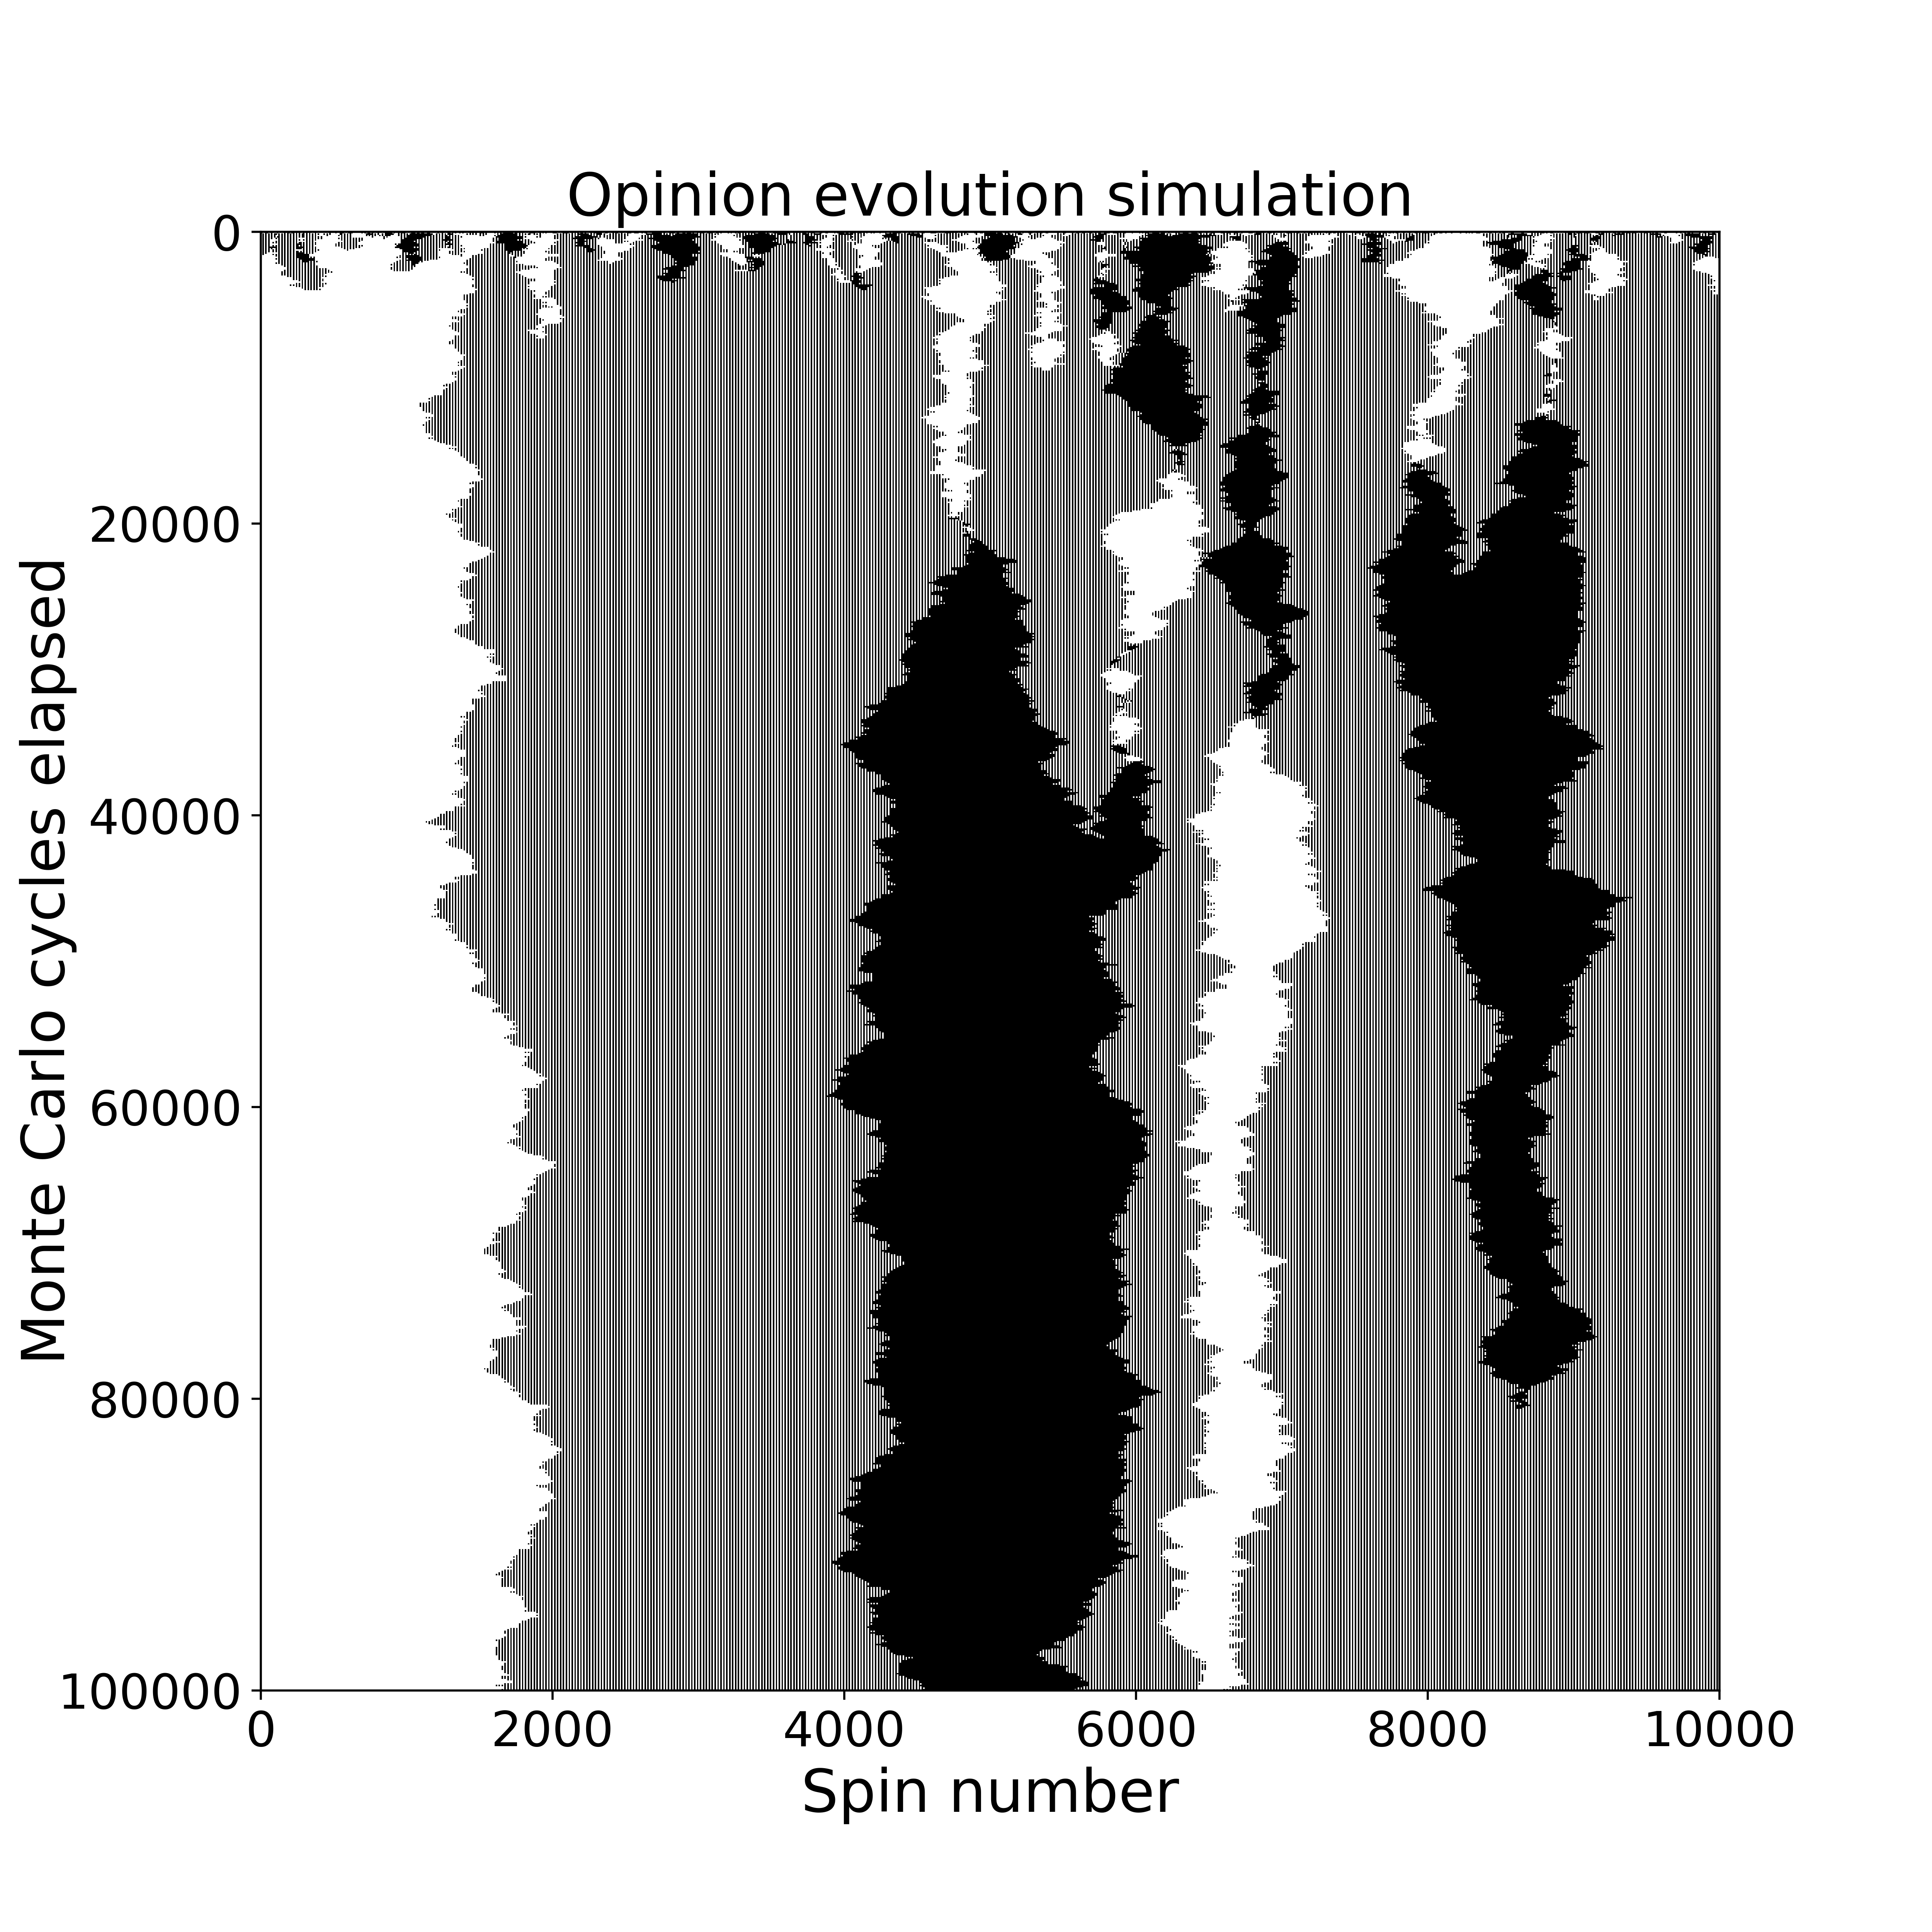
\includegraphics[width=1.0\textwidth]{large.png}}
 \caption{Experiment with 100000 spins. Each horizontal line of pixels in the picture represents the configuration of spins at a given moment. Time evolves from the initial random ordering at the top and downwards. As can be seen the random configuration quickly reshuffles into a sequence of clusters, with black and white representing the AAAA and BBBB states and the ordered stripes the ABAB state. At the bottom, after 100000 MC-cycles, each containing 100000 random draws, it is still not settled. As can be seen any alteration of state occurs at the border of a cluster. We can also see clusters that are fully white or black that narrow in, with the striped state on either side, to regrow in the opposite color. There are, however, no sign that the border between the striped and a black or white state spontaneously gives rise to the other color. }
 \label{fig:large}
\end{figure}



With a system of 4 spins we can write out the 16 possible system permutations and investigate the outcomes. The way we have implemented the code the system matrix is padded with one position to the left and one to the right. These positions serve to make it possible to apply the rules on the border of the system, but the padded positions are not a part of the system.  We can draw any of the three first of the four positions when we want to apply the rules, but the fourth position can not be drawn, as it would require multiplication with a position outside the system to establish what rule to apply. For clarity we repeat the rules:

\begin{enumerate}
\item if $S_iS_{i+1}=1$ then $S_{i-1}$ and $S_{i+2}$ take the direction of the pair (i,i+1),

\item if $S_iS_{i+1}=-1$ then $S_{i-1}$ takes the direction of $S_{i+1}$ and $S_{i+2}$ the direction of $S_i$. 
\end{enumerate}



%A couple of examples :


%\begin{align*}
    % \text{ 1 1 1 1} & \quad\xrightarrow[i=1]{\text{\space\space\space\space\space\space\space}}\quad\text{ 1 1 1 1} & &\\
    % \text{-1 1 1 1} & \quad\xrightarrow[i=1]{\text{rule 2}} \quad\text{ 1 1-1 1} & &\\
    % \text{or}       & \quad\xrightarrow[i=2,3]\quad\text{\space\space\space\space -1 1 1 1} & &\\
    % \text{ 1 -1 1 1} & \quad\xrightarrow[i=1,3]\quad\text{\space\space\space\space 1 -1 1 1} & &\\
    % \text{or}       & \quad\xrightarrow[i=2]{\text{rule 2}}\quad\text{  1 -1 1 -1} & &\\
    % \text{ 1 1 -1 1} & \quad\xrightarrow[i=1]{\text{rule 1}}\quad\text{ 1 1 1 1} & &\\
    % \text{or}       & \quad\xrightarrow[i=2]{\text{rule 2}}\quad\text{  -1 1 -1 1} & &\\
    % \text{or}       & \quad\xrightarrow[i=3]{\text{\space\space\space\space\space\space\space}}\quad\text{  1 1 -1 1} & &\\
    %\text{ 1 1 1 -1} & \quad\xrightarrow[i=1]{\text{rule 1}}\quad\text{ 1 1 1 -1} & &\\
    %\text{or}       & \quad\xrightarrow[i=2]{\text{rule 1}}\quad\text{  1 1 1 1} & &\\
    %\text{or}       & \quad\xrightarrow[i=3]{\text{rule 2}}\quad\text{  1 -1 1 -1} & &\\
    %\text{-1 -1 1 1} & \quad\xrightarrow[i=1]{\text{rule 1}} \quad\text{ -1 -1 -1 1} & &\\
    %\text{or}       & \quad\xrightarrow[i=2]{\text{rule 2}}\quad\text{  1 -1 1 -1} & &\\
    %\text{or}       & \quad\xrightarrow[i=3]{\text{rule 1}}\quad\text{  -1 1 1 1} & &\\
    % \text{ 1-1 1-1} & \\
    % \text{-1 1 1 1} & \quad\xrightarrow[i=1]{\text{rule 2}} \quad\text{-1 1-1 1} & &\\
    % \text{or}       & \quad\xrightarrow[i=2]{\text{rule 1}} \quad\text{ 1 1 1 1} & &\\
    % \text{ 1-1 1 1} & \quad\xrightarrow[i=1]{\text{rule 2}}\quad\text{ 1-1 1-1} & &\\
    % \text{or}       & \quad\xrightarrow[i=2]{\text{rule 1}} \quad\text{ 1 1 1 1} & &\\
    % \text{ 1 1-1 1} & \quad\xrightarrow[i=2]{\text{rule 2}}\quad\text{-1 1-1 1} & &\\
    % \text{ 1 1 1-1} & \quad\xrightarrow[i=3]{\text{rule 2}}\quad\text{ 1-1 1-1} & &\\
    % \text{-1-1 1 1} & \quad\xrightarrow[i=2]{\text{rule 2}}\quad\text{ 1-1 1-1} & &\\
    % \text{or}       & \quad\xrightarrow[i=3]{\text{rule 1}}\quad\text{-1 1 1 1} \quad\xrightarrow[i=2]{\text{rule 1}}\quad\text{ 1 1 1 1} &\\
    % \text{or}       & \quad\xrightarrow[i=3]{\text{rule 1}}\quad\text{-1 1 1 1} \quad\xrightarrow[i=1]{\text{rule 2}}\quad\text{-1 1-1 1} &\\
    % \text{ 1-1-1 1} & \quad\xrightarrow[i=1]{\text{rule 2}}\quad\text{ 1-1 1 1} \quad\xrightarrow[i=2]{\text{rule 2}}\quad\text{ 1-1 1-1} &&\\
    % \text{or}       & \quad\xrightarrow[i=1]{\text{rule 2}}\quad\text{ 1-1 1 1} \quad\xrightarrow[i=3]{\text{rule 1}}\quad\text{ 1 1 1 1} &&\\
%\end{align*}




%Joachims version
The states and their resulting outcomes, where we interpret A as -1 and B as 1:


 \begin{align*}
     \text{ 1 1 1 1} && \text{BBBB, }p=1/16 \\
     \text{ 1-1 1-1} && \text{BABA, }p=1/16 \\
     \text{-1 1 1 1} & \quad\xrightarrow[i=1]{\text{rule 2}}\quad\text{-1 1-1 1} & \text{ABAB, }p=1/32\\
     \text{or}       & \quad\xrightarrow[i=2]{\text{rule 1}}\quad\text{ 1 1 1 1} & \text{BBBB, }p=1/32\\
     \text{ 1-1 1 1} & \quad\xrightarrow[i=2]{\text{rule 2}}\quad\text{ 1-1 1-1} & \text{BABA, }p=1/32\\
     \text{or}       & \quad\xrightarrow[i=3]{\text{rule 1}}\quad\text{ 1 1 1 1} & \text{BBBB, }p=1/32\\
     \text{ 1 1-1 1} & \quad\xrightarrow[i=2]{\text{rule 2}}\quad\text{-1 1-1 1} & \text{ABAB, }p=1/32\\
     \text{or}       & \quad\xrightarrow[i=1]{\text{rule 1}}\quad\text{ 1 1 1 1} & \text{BBBB, }p=1/32\\
     \text{ 1 1 1-1} & \quad\xrightarrow[i=3]{\text{rule 2}}\quad\text{ 1-1 1-1} & \text{BABA, }p=1/32\\
     \text{or}       & \quad\xrightarrow[i=2]{\text{rule 1}}\quad\text{ 1 1 1 1} & \text{BBBB, }p=1/32\\
     \text{-1-1 1 1} & \quad\xrightarrow[i=2]{\text{rule 2}}\quad\text{ 1-1 1-1} & \text{BABA, }p=1/32\\
     \text{or}       & \quad\xrightarrow[i=3]{\text{rule 1}}\quad\text{-1 1 1 1} \quad\xrightarrow[i=2]{\text{rule 1}}\quad\text{ 1 1 1 1} &\text{BBBB, }p=1/64\\
     \text{or}       & \quad\xrightarrow[i=3]{\text{rule 1}}\quad\text{-1 1 1 1} \quad\xrightarrow[i=1]{\text{rule 2}}\quad\text{-1 1-1 1} &\text{ABAB, }p=1/64\\
     \text{ 1-1-1 1} & \quad\xrightarrow[i=1]{\text{rule 2}}\quad\text{ 1-1 1 1} \quad\xrightarrow[i=2]{\text{rule 2}}\quad\text{ 1-1 1-1} &\text{BABA, }p=1/64\\
     \text{or}       & \quad\xrightarrow[i=1]{\text{rule 2}}\quad\text{ 1-1 1 1} \quad\xrightarrow[i=3]{\text{rule 1}}\quad\text{ 1 1 1 1} &\text{BBBB, }p=1/64\\
     \text{or}       & \quad\xrightarrow[i=2]{\text{rule 1}}\quad\text{ -1-1-1-1} &\text{AAAA, }p=1/32\\
 \end{align*}




The remaining half of outcomes is given by simply inverting the signs of the states above. 

 As can be seen here the three fixed points (AAAA,BBBB, ABAB) occurs with fractions $(1/16+4/34+2/64=1/4)$,  $(1/16+4/32+4/64=1/4)$ and $(2/16+10/32+4/64=1/2)$ respectively. This is in line with the expected result. It is, however, not given that a system of 4 spins can reproduce the dynamics of a larger system. 
 
What can be derived is that no angle of attack will lead rise to alteration once the AAAA, BBBB or ABAB state is established, meaning that even for any system size, alterations can only occur at sites not in a cluster of settled states or at sites that border clusters. 

Further, regardless of system size, we see that at any border between clusters there will be two possible sites that can lead to change, determining whether one cluster or the other is growing, or whether the third emerges in between. The border AAABBB can alter to AABBBB  or AAAABB by rule 1 in one step, or it can alter to ABABAB by rule 2. As one out of the three possible sites at the border that can alter it leads to the formation of an undecided cluster between the decided, such borders, between black and white, are inherently short lived, as they sooner or later turn into an imposing cluster of the striped state. This is in fact the key to the probability distribution of final settled states, as the border between two decided states can and will give rise to a divided cluster spawning, but the border between the divided and one of the decided states cannot give rise to the other decided state. Another way of interpreting it is that the striped state actually represents two different fixed point cluster formations, namely both the ABAB and the BABA, which each have a 1/4 probability of being the final steady fixed point.

Borders between divided and decided clusters can be shifted to either side with equal probability. If a decided cluster is surrounded on both sides by undecided clusters that are not in phase it can be annihilated down to a two spin size and either regrow or turn into an oppositely decided cluster. See Figure \ref{fig:close}, which is a close up from Figure \ref{fig:corr1}. 

\begin{figure}[H]
 \centerline{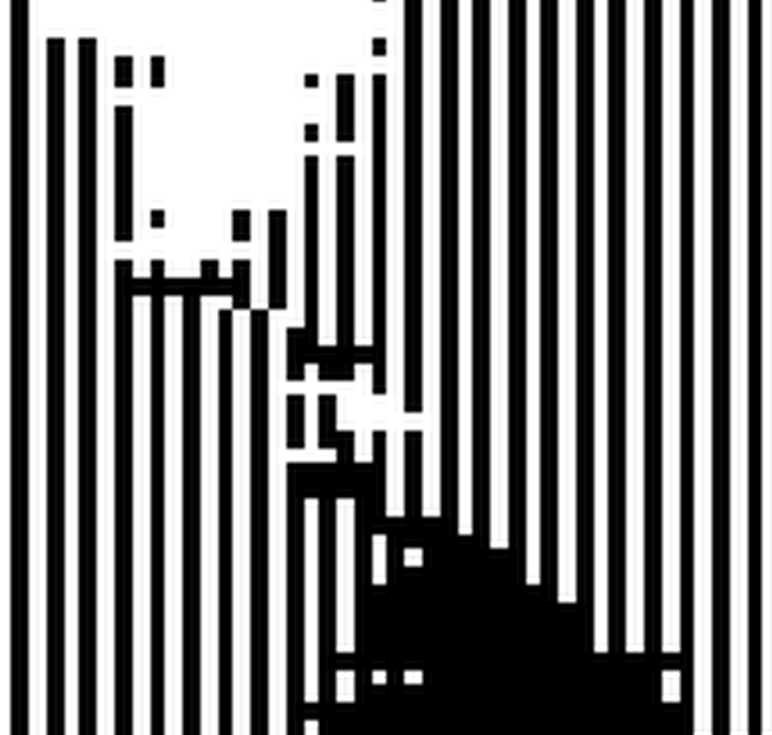
\includegraphics[width=0.5\textwidth]{Close.png}}
 \caption{Close up from Figure \ref{fig:corr1}. The divided clusters on either side are out of phase. For either of the surrounding divided clusters to win ultimately, the other must first be consumed by one of the decided states, or by an in-phase divided cluster from the other side.}
 \label{fig:close}
\end{figure}



In Figures \ref{fig:equal}-\ref{fig:white} we can see simulations that ended up in the three possible final states. Experiments that took longer to settle where chosen to display more of the possible dynamics.


\begin{figure}[H]
 \centerline{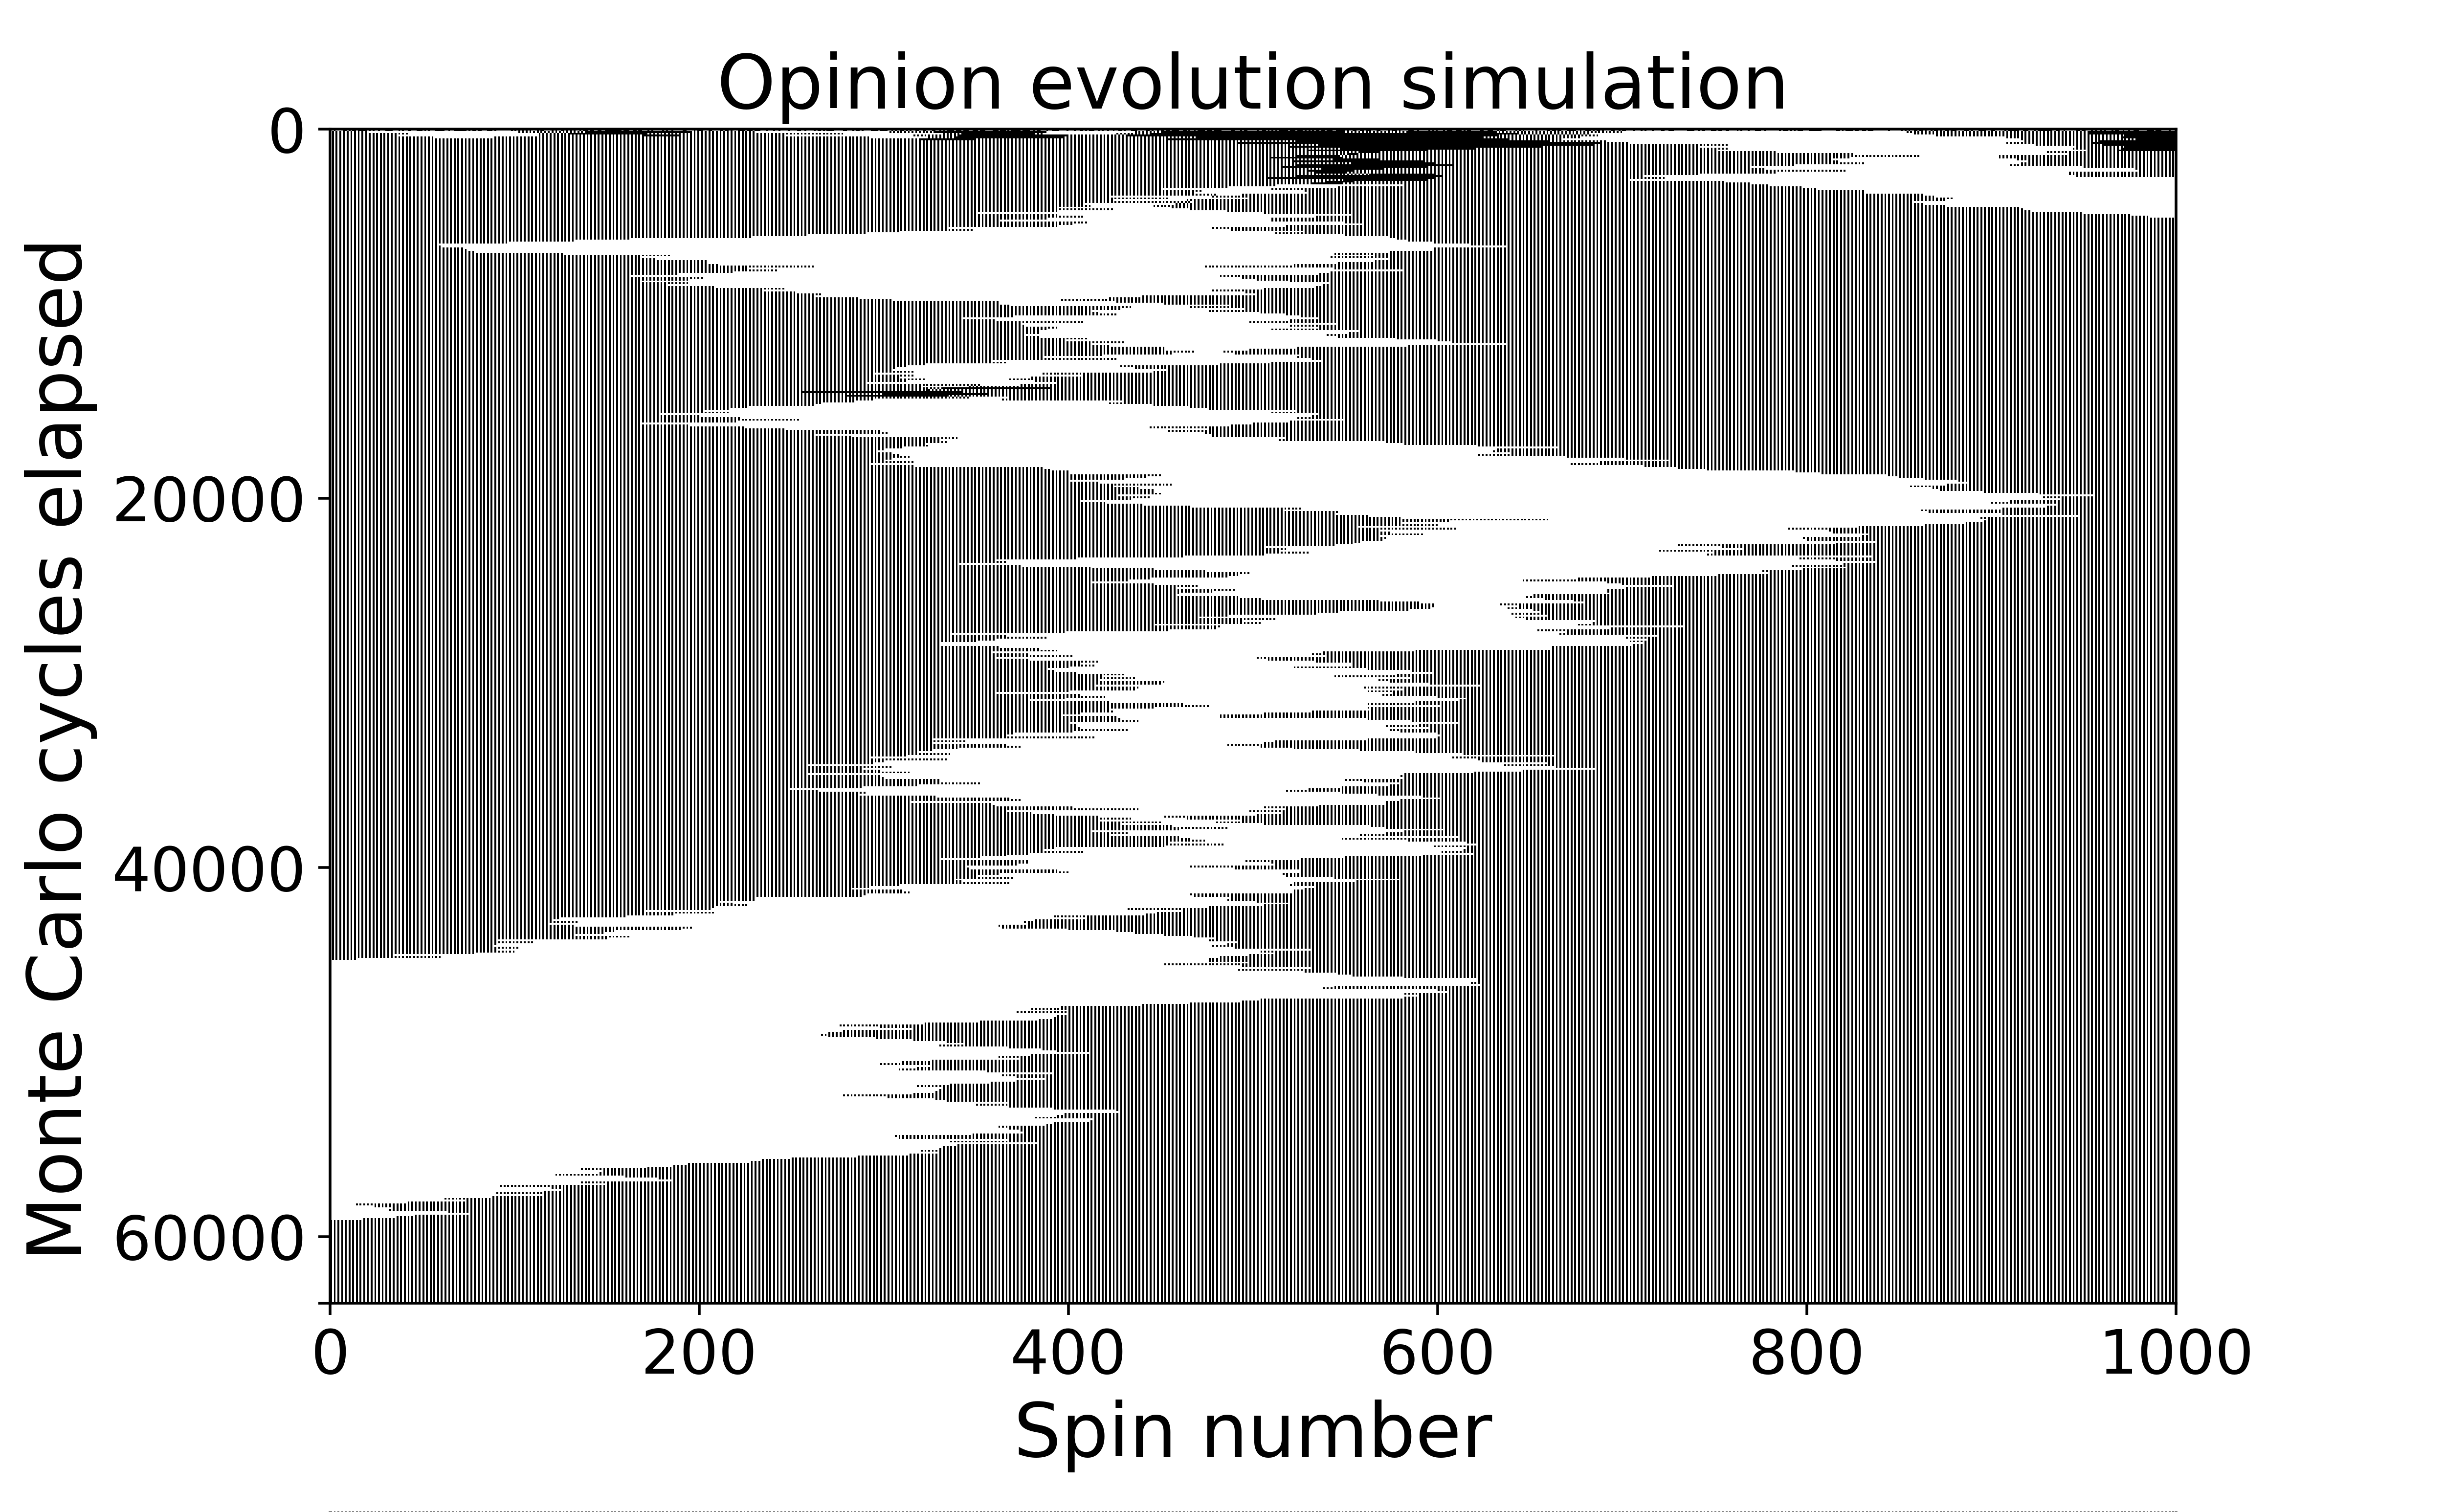
\includegraphics[width=1.0\textwidth]{equal.png}}
 \caption{Experiment that settles in the equally divided state. Early in the simulation all three states have some clusters, but at a quite early point it seems to stand between the white and the divided state.}
 \label{fig:equal}
\end{figure}

\begin{figure}[H]
 \centerline{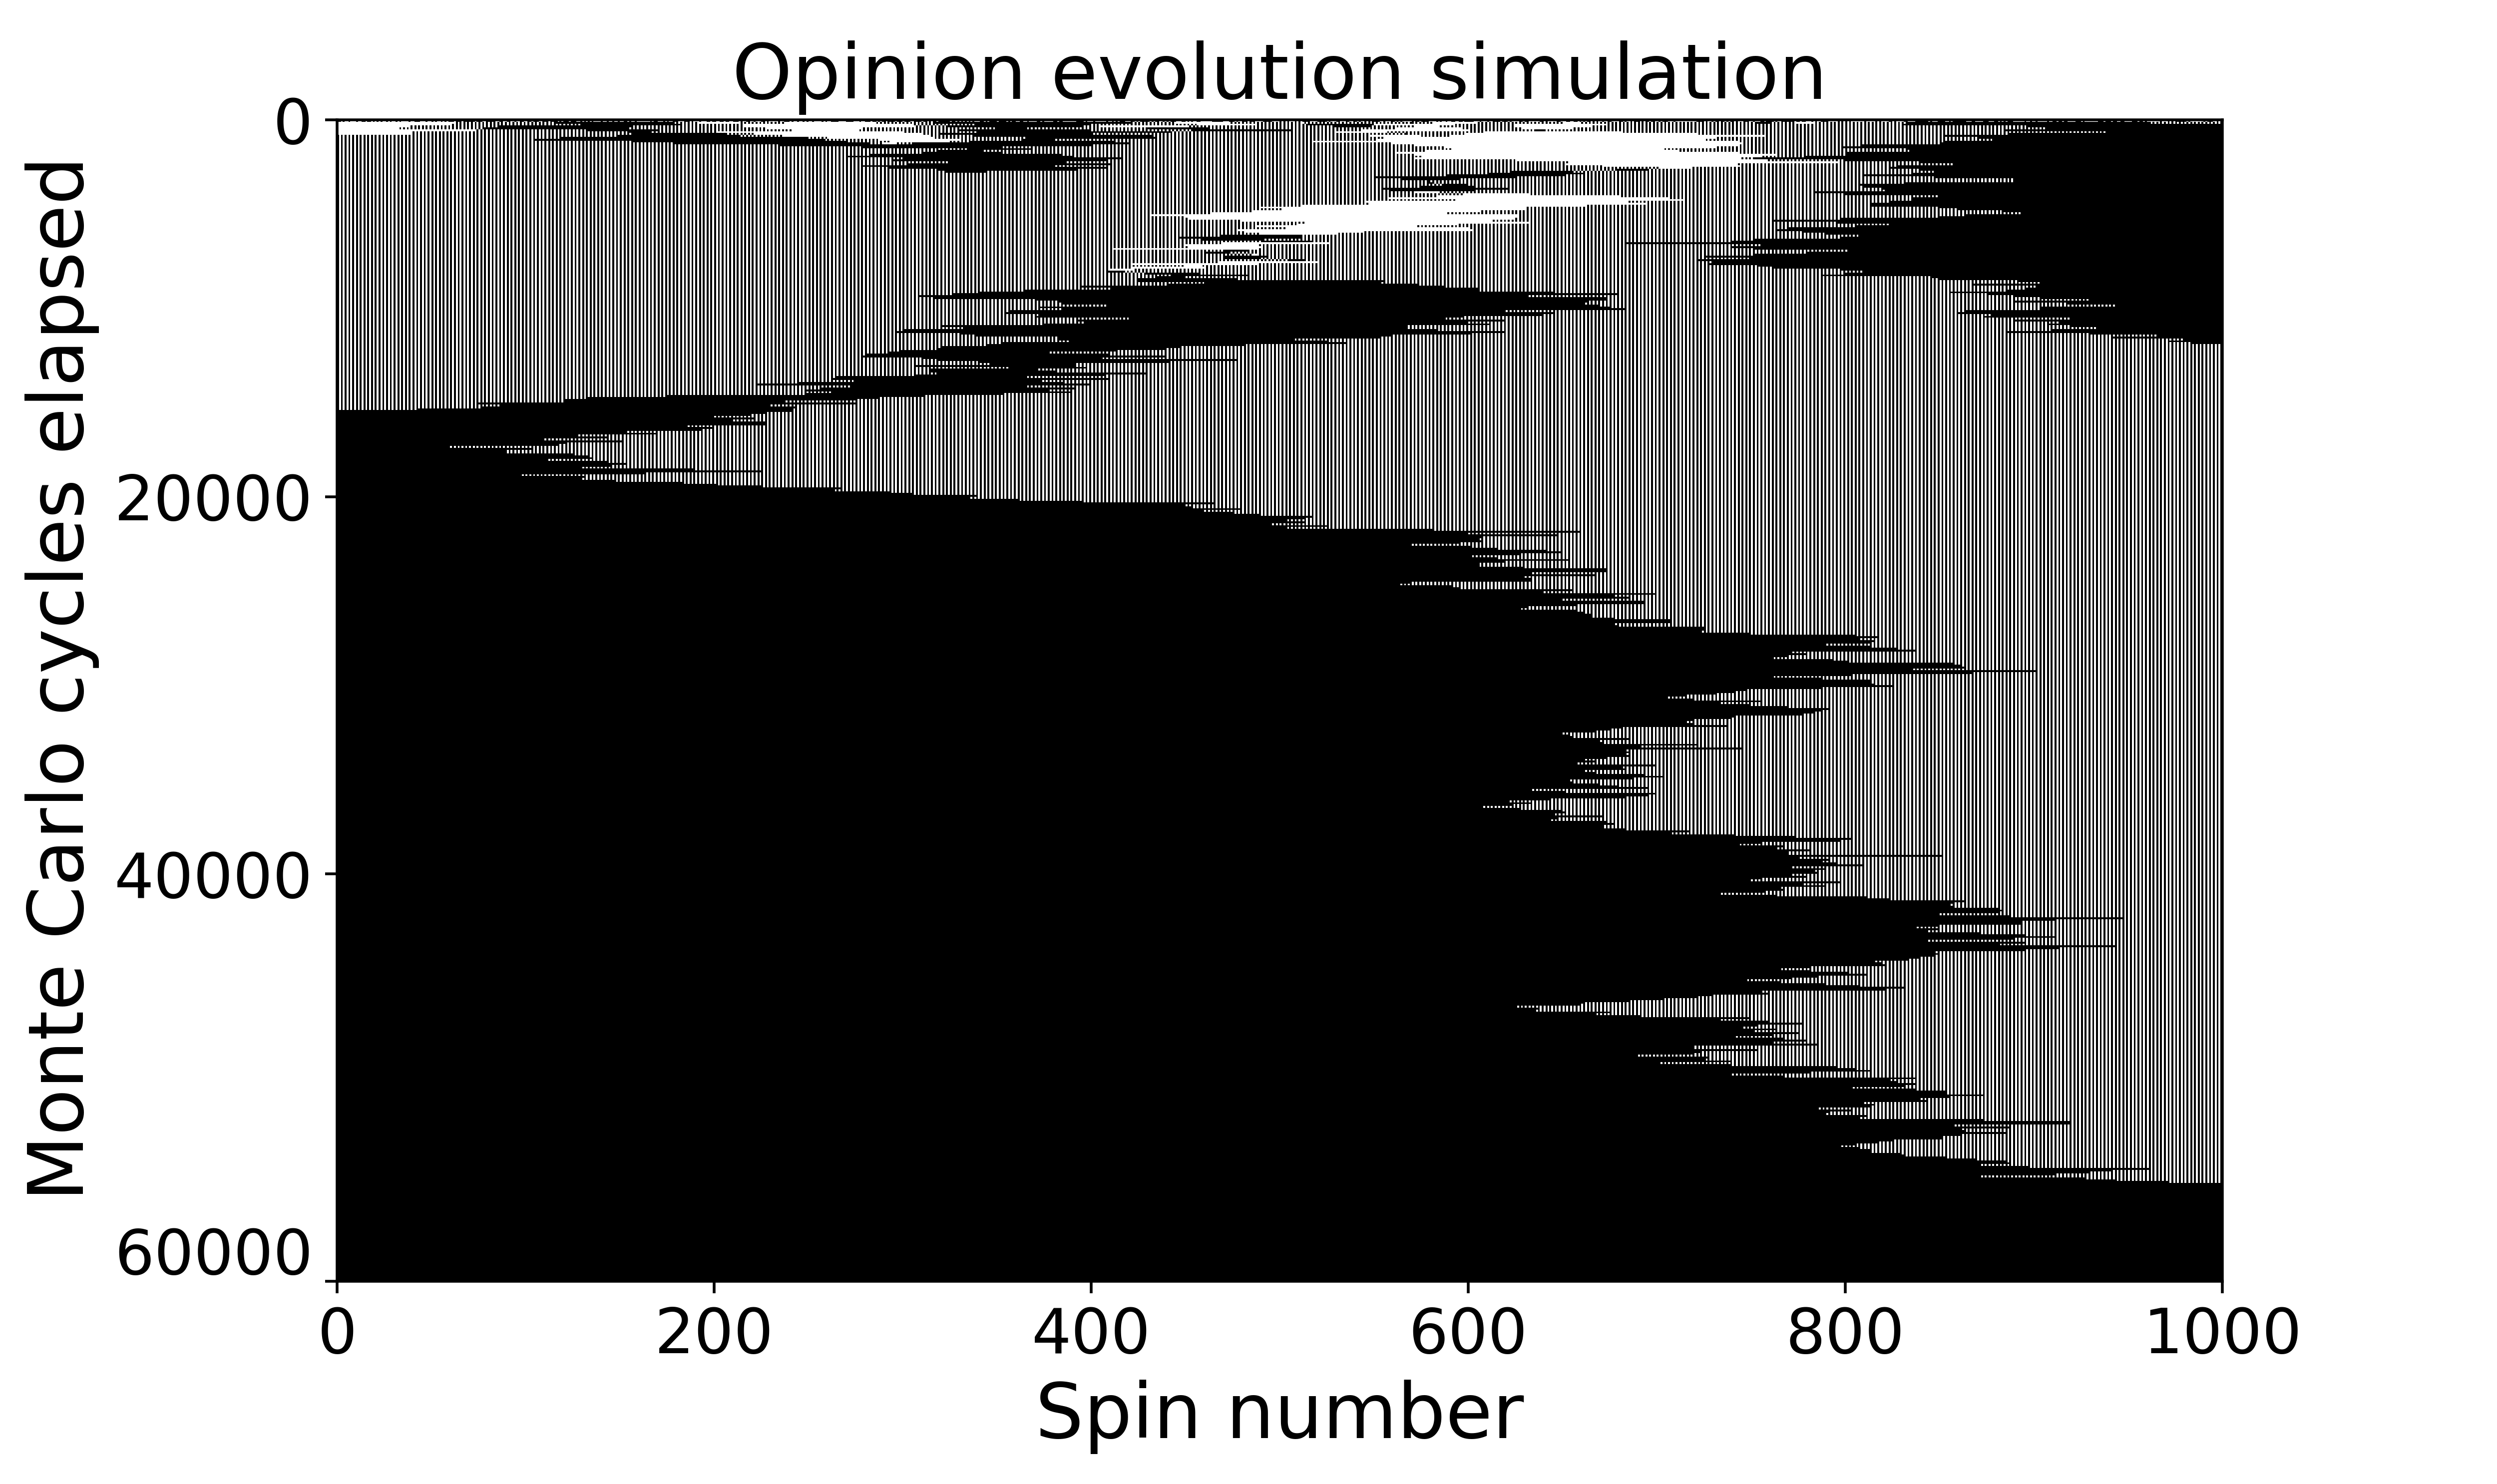
\includegraphics[width=1.0\textwidth]{black.png}}
 \caption{Realization resulting in an all black fixed state.}
 \label{fig:black}
\end{figure}

\begin{figure}[H]
 \centerline{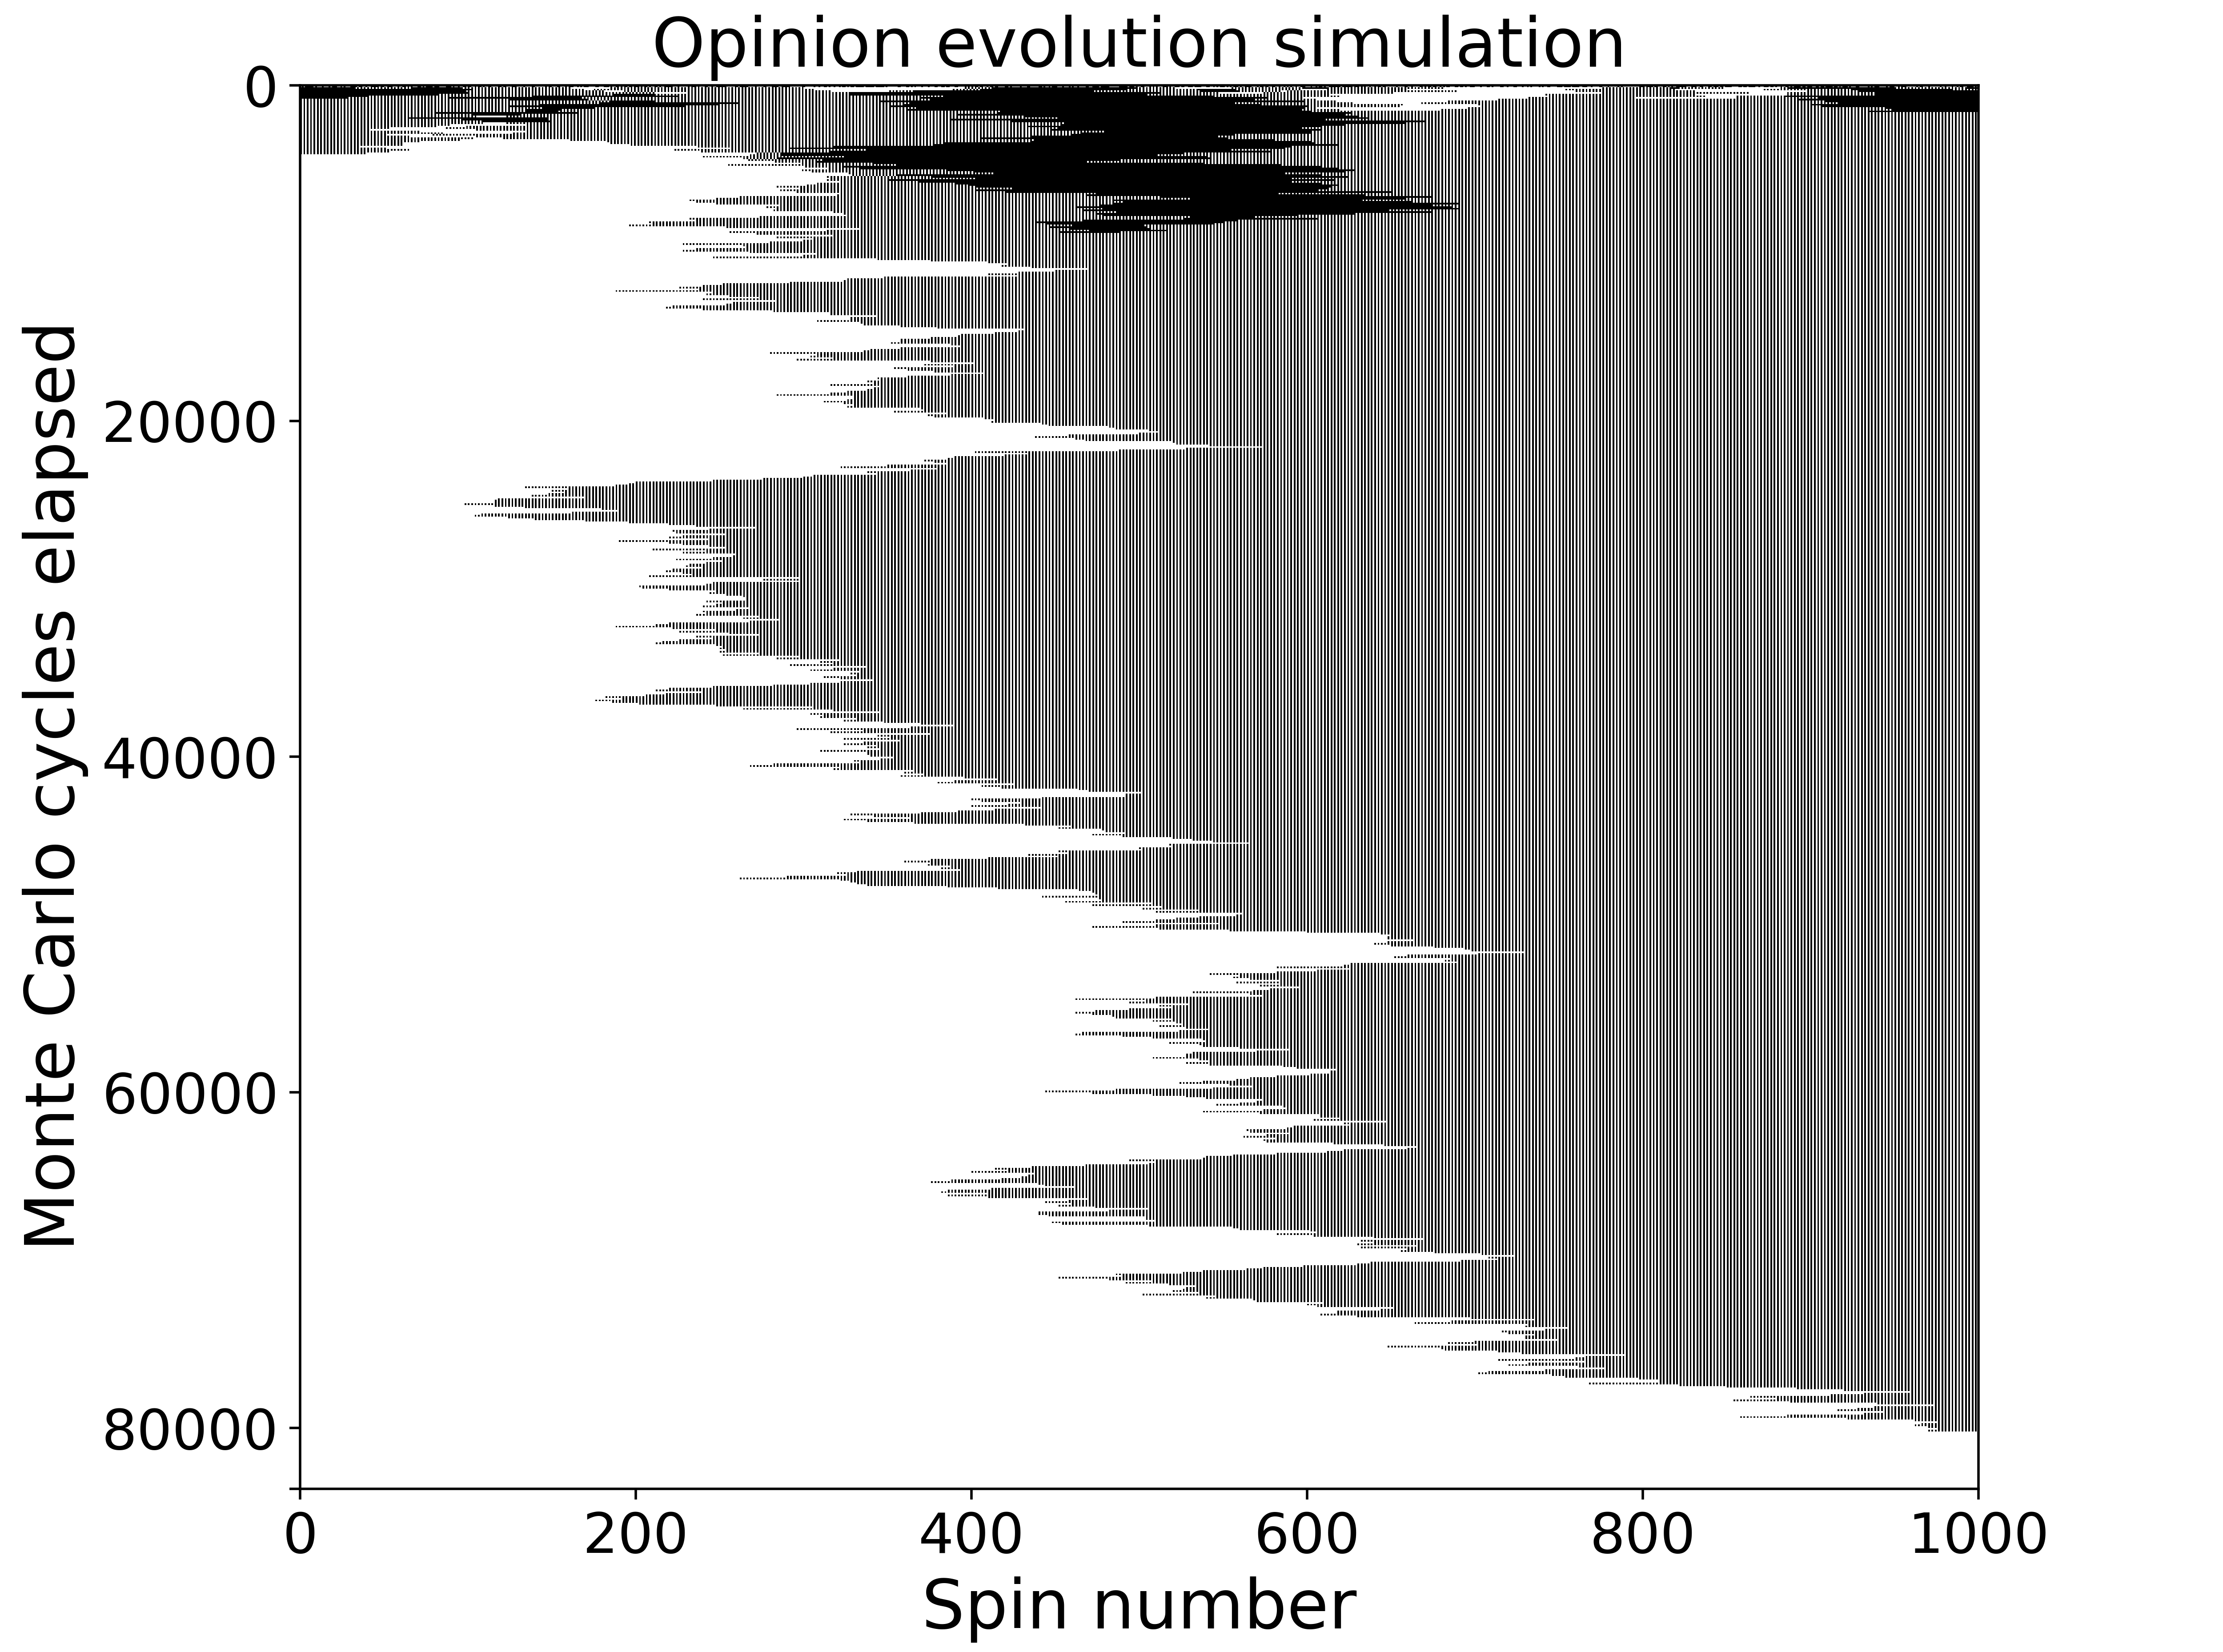
\includegraphics[width=1.0\textwidth]{white.png}}
 \caption{Realization resulting in an all white fixed state.}
 \label{fig:white}
\end{figure}

As the figures suggest the simulations end up being a 50-50 proposition between the divided and one of the decided states. Having a cluster along a wall gives an advantage, as the cluster cannot be attacked from this side, so any configuration that can establish it self at both sides has an advantage, but as Figure \ref{fig:black} shows, this need not be decisive. 


To determine the probability distribution between the three possible final outcomes we run 1000 systems over $10^5$ MC-cycles of $1000$ random draws. With the assumption that every system would reach a fixed state. Upon running the experiments we found that a number of simulations did in fact not reach the fixed state. The final mean magnetisation at the end of each is appended to a list. The resulting distribution came up as: 
\begin{itemize}
    \item Unresolved fraction 37/1000
    \item AAAA fraction 260/1000 $\rightarrow$ normalised fraction 0.49
    \item BBBB fraction 229/1000 $\rightarrow$ normalised fraction 0.24
    \item ABAB fraction 474/1000 $\rightarrow$ normalised fraction 0.27
\end{itemize}

This results stand as  a verification the probability distribution from  \cite{opinion}. In Figure \ref{fig:hist} we show the distributions from experiments with different system sizes that further strengthens this result.

\begin{figure}[H]
 \centerline{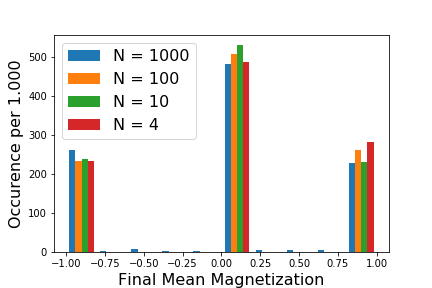
\includegraphics[width=0.8\textwidth]{histogram.png}}
 \caption{The distribution of mean magnetization after $100N$ MC-cycles for 1000 realizations with different system sizes $N$. As can be seen the distributions follow the predictions from \cite{opinion} quite closely.}
 \label{fig:hist}
\end{figure}



\subsection{Magnetization and social mood.}
In Figure \ref{fig:mag} we see the time evolution of the mean decision or magnetization, as per Equation \ref{eq:mag}, of the three systems from Figures \ref{fig:equal}-\ref{fig:white}.  
\begin{figure}[H]
 \centerline{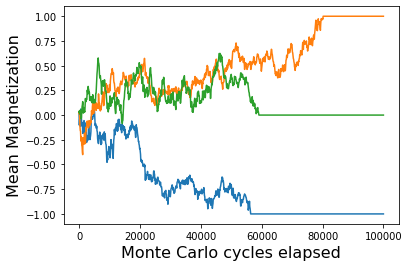
\includegraphics[width=0.8\textwidth]{mag.png}}
 \caption{The evolution mean magnetization as a function of MC-cycles, for the systems illustrated in Figures \ref{fig:equal}-\ref{fig:white}.}
 \label{fig:mag}
\end{figure}

As can be seen by combining the plots the field is only truly open while all three cluster-configurations are represented, unless there are at least two divided clusters that are out of phase remaining. As soon as one of the decided clusters is exterminated  and the divided are in phase, it stands between the remaining decided and the undecided, and the magnetization stays firmly in the positive or negative, to finally converge to one of the poles or to 0. Hypothetically a show down between decided states can occur, but since one third of the possible transitions involves the emergence of a divided state in between, this is only hypothetical for any system involving more than a handful of spins.



\subsection{Time correlation of the magnetization}
To study the time correlation of the magnetization we run a simulation of $10^4$ spins and record the state after every one of $10^4$ MC-cycles. The realization can be seen in Figure \ref{fig:corr1}.

\begin{figure}[H]
 \centerline{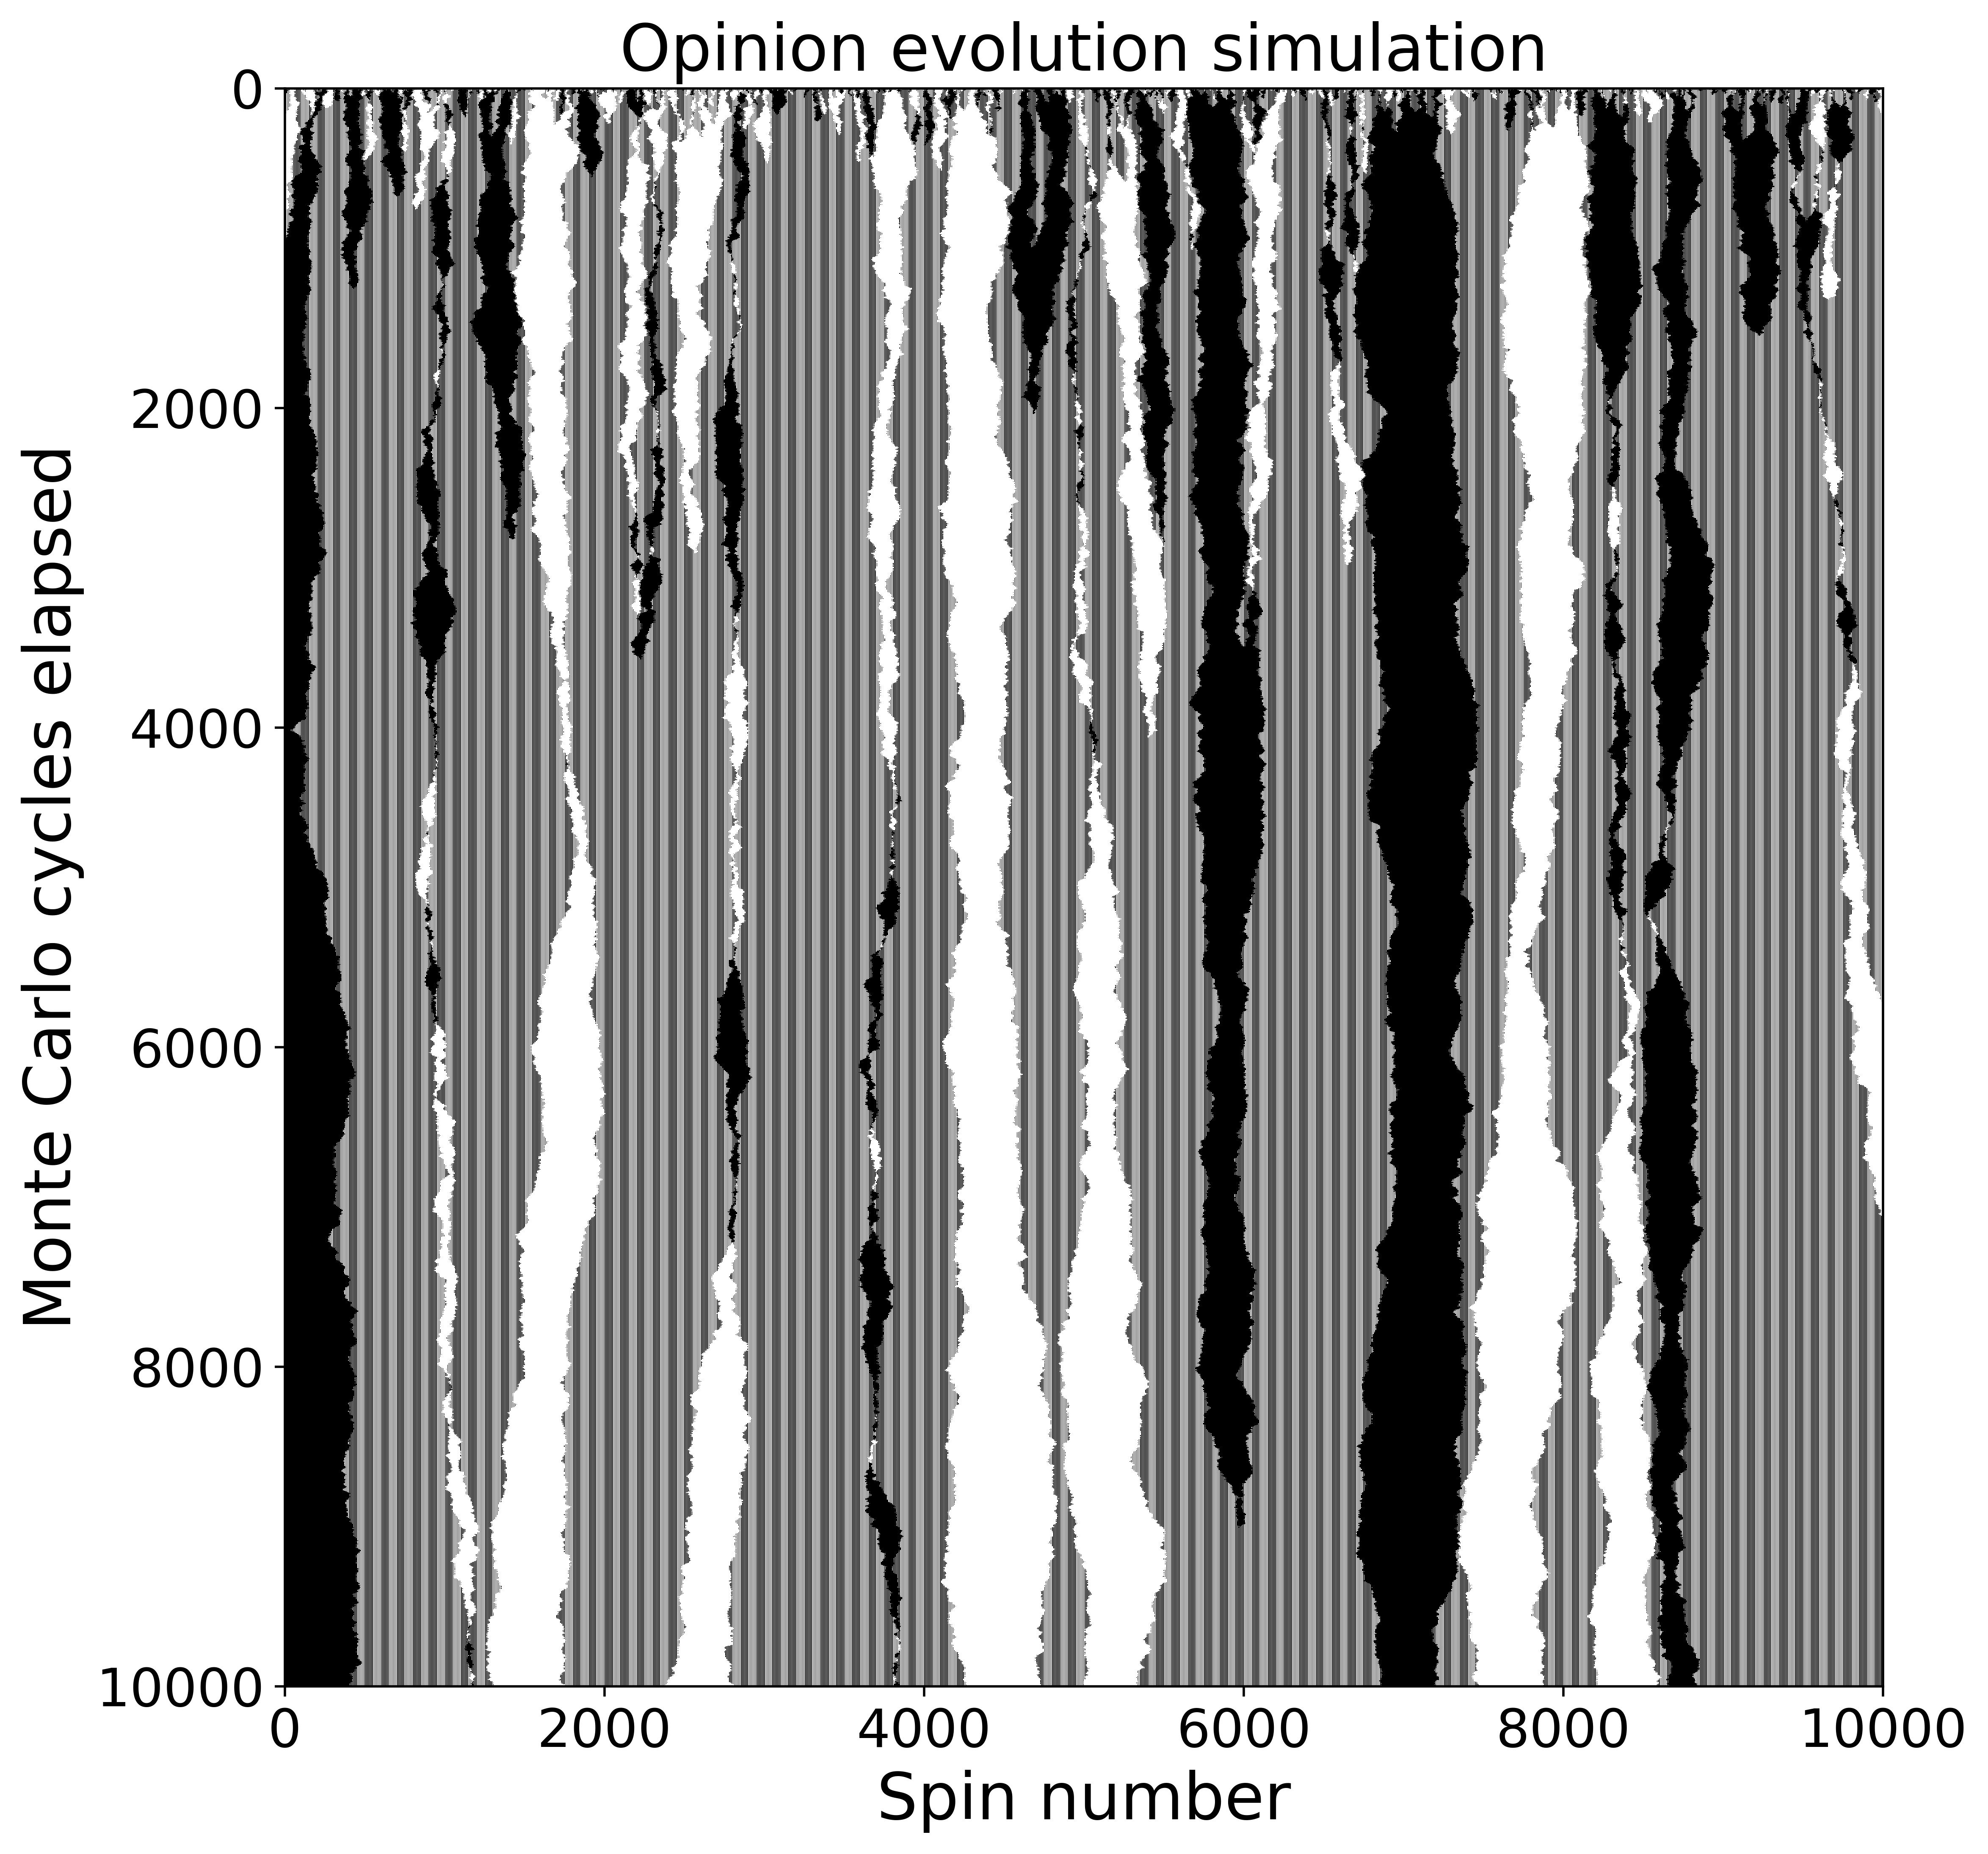
\includegraphics[width=0.8\textwidth]{bigcorrelate.png}}
 \caption{System with $N=10^4$ spins simulated over $10^4$ MC-cycles, recorded after every cycle. The in-detail look at the beginning of the experiment reveals a much larger span in dynamics than the later stages of the simulations.}
 \label{fig:corr1}
\end{figure}

In Figure \ref{fig:corr2} we see the corresponding time evolution of the mean magnetization, from Equation \ref{eq:mag}. 

\begin{figure}[H]
 \centerline{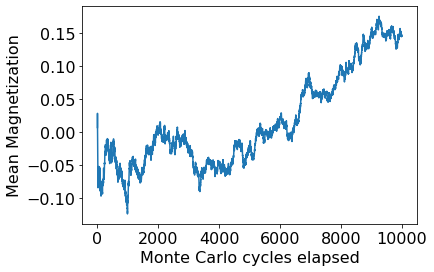
\includegraphics[width=0.8\textwidth]{corrmag.png}}
 \caption{The evolution of the mean magnetization}
 \label{fig:corr2}
\end{figure}


\begin{figure}[H]
 \centerline{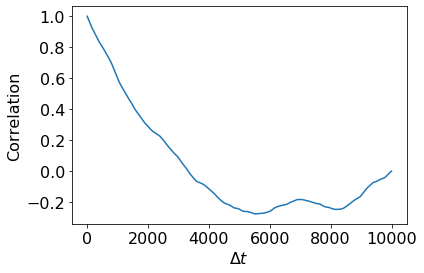
\includegraphics[width=0.8\textwidth]{corrCurv.png}}
 \caption{The time autocorrelation of the mean magnetization. As can be seen the correlation decreases rapidly with increased $\Delta t$. }
 \label{fig:corr3}
\end{figure}

 We use Equation \ref{eq:corr} to quantify the time correlation of the mean magnetisation. The correlation of magnetization illustrates how the distribution of spin, or opinion, at one time, is significant for the state at some other time. In Figure \ref{fig:corr3} we see the time correlation of the magnetization.  As can be seen the correlation drops rapidly, meaning that the initial state of the system gives little information about how it evolves. 

To get an idea of how the system affects individual spins we measure how many MC-cycles elapse between decisions for each in the realisation from Figure \ref{fig:corr1}. The measurements are basically of the lengths of the unbroken vertical lines, pixel column by pixel column, but excluding the lines that start from the top or end at the bottom. By far the most common interval between decisions was one MC-cycle, accounting for a total of 27\% of the measured intervals, suggesting that the probability for a spin to again change its direction immediately after having done so is high. This can also be understood intuitively. The realizations show that the entire domain quite quickly organizes itself into a sequence of clusters of fixed states after initiation. Thereafter only the sites at a border between cluster can be flipped, meaning that if a site is flipped, it is one of a limited number of sites that can be flipped again or it is close to a site that can be flipped. It can however, remain unchanged also, and any interval that spans the length of the experiment is possible. Here it is also worth noting that every MC-cycle contains as many random draws as there are spins, so any individual can be flipped multiple times and borders between clusters can also move during one MC-cycle.

By studying the measurements we can further interpret the distribution of intervals. Figure \ref{fig:power} shows the distribution of $P(\tau)$ as a loglog plot and the fitted line shows a power law with an exponent of -3/2, so we have $P(\tau)\sim \tau^{-3/2}$ as found by \cite{opinion}.


\begin{figure}[H]
 \centerline{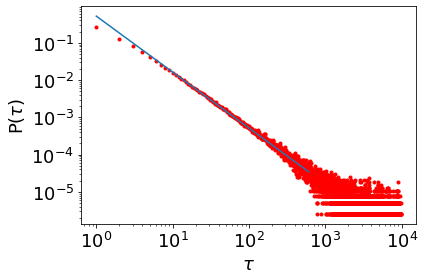
\includegraphics[width=0.8\textwidth]{power1.png}}
 \caption{Loglog plot of $P(\tau)$ vs $\tau$. The fitted line has a slope of -1.50, with data included for $\tau$ up to 800 MC-cycles. If we include the remaining data the slope flattens considerably and deviates from the data, it is no longer reasonable to assume a power law. } 
 \label{fig:power}
\end{figure}


\subsection{Initial conditions}
Katarzyna Sznajd-Weron and Józef Sznajd also considered how the initialization of the system affects the probability distribution of final fixed states \cite{opinion}. In Figure \ref{fig:cb} we have reproduced their result by considering a case where we have initiated our system with a controlled fraction of sites set as B and sites set as A, through the parameter $c_B$, the concentration of B.


\begin{figure}[H]
 \centerline{\includegraphics[width=0.8\textwidth]{cbdist.png}}
 \caption{The distributions of outcomes for 1000 trials with 9 different levels of $c_B$. for efficiency the runs were only conducted with 100 spins. Random sampling with 1000 spins matched the distribution found here. We tried both with random shuffling and with the first $N*c_B$ spins set to B and the remaining to A, with indistinguishable results. }
 \label{fig:cb}
\end{figure}

The plot confirms the findings of \cite{opinion} as well as the observation that $c_B$ must exceed 0.7 to make more than half the outcomes turn out BBBB.


The article \cite{opinion} found that the distribution of $P(\tau)$ was not affected by the initial conditions. We confirmed this by random sampling and the result is in tune with our intuition of the system, which we will expand more on in the following section.


\subsection{Information Noise}
We also consider the effect of introducing a weak probability that the rules are disobeyed when applied. The realisation is done by introducing a probability, $p$, that the affected spins in a draw, instead of following the rules, chose randomly between A and B with equal probability. 

In Figure \ref{fig:noise1} we see realisations with different probabilities, $p$, that the drawn spins choose to randomly decide. In \cite{opinion} they considered how small the probability would have to be, for a determined system to decidedly not be thrown out of the condition. They illustrated the case by plotting the mean magnetization evolution for different $p$. They conclude that there is some limit $p*\in [10^{-6},10^{-5}]$ below which the system remains ordered, While for larger $p$ the system may divert to disorder. We find similar results, as seen in the figure with the same set selection of values for $p$, but we are not entirely in agreement about the limit $p*$, as any introduction of a disruptive spin in a fixed cluster may lead to the formation of a fully disordered system, which in turn may then settle into any of the fixed states. 

\begin{figure}[H]
 \centerline{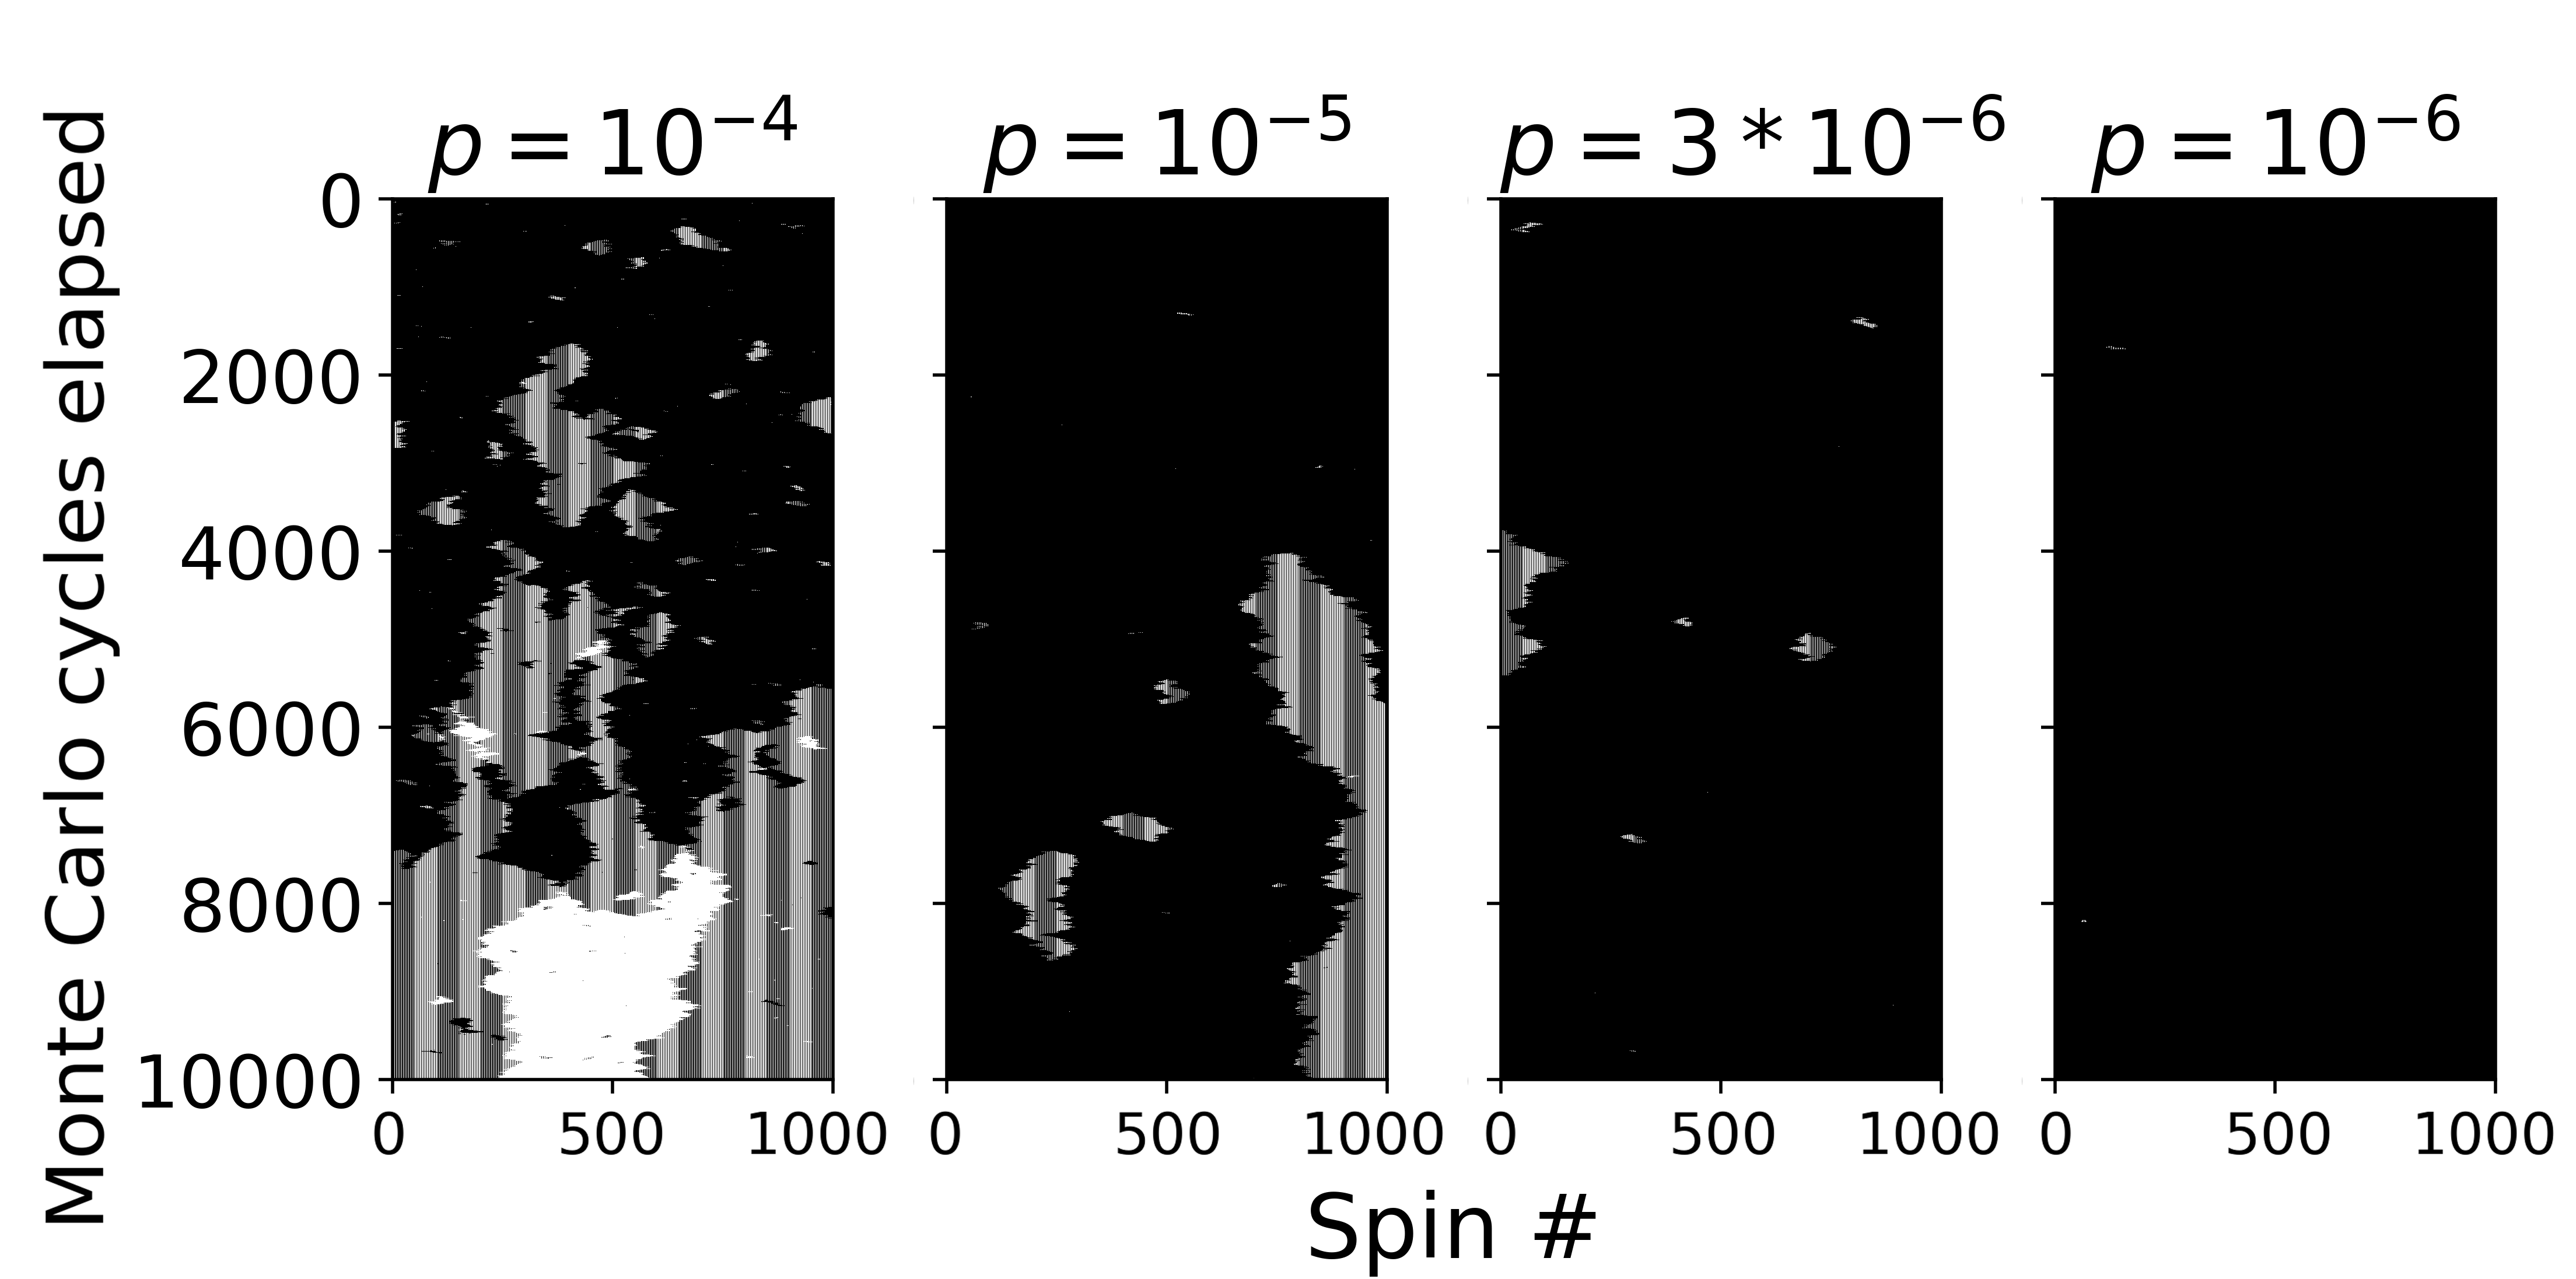
\includegraphics[width=1.0\textwidth]{noise2.png}}
 \caption{Time evolution for systems with $N=1000$ spins, all initialized as B, with decreasing probability, $p$, for drawn spins to disobey the rules. Even though it is hard to see in the figure, the lowest probability (on the right) also gives rise to occasional disruptive "white pixels".}
 \label{fig:noise1}
\end{figure}



In the article \cite{opinion} the authors also consider how this modification of the rules affect the mean decision time. In Figure \ref{fig:noise2} we have reached a matching result, where we also find that the probability for a longer period between decisions decreases with the introduced system noise.


\begin{figure}[H]
 \centerline{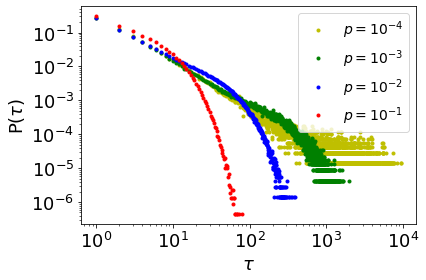
\includegraphics[width=0.8\textwidth]{power3.png}}
 \caption{The time evolution for systems that allow for the drawn spins to disobey the rules, with a probability $p$.}
 \label{fig:noise2}
\end{figure}

The time between decision, without noise, was found to not be dictated by initial conditions or concentration, but rather by the rules. As stated before, as soon as the system is organized into a sequence of clusters the rules, without noise, only allows for spins to flip at the border between clusters. As the spins that have just been flipped are still at, or next to the border, they are likely to be flipped again. However, if the border shifts away, the spins are removed from the border and cannot be flipped as they remain inside a cluster. With the introduced noise also the spins firmly inside clusters may be flipped and the system changes more rapidly. Equation \ref{eq:tau2} shows the modified law for the distribution of $P(\tau)$, as deduced by \cite{opinion}. 


\begin{equation}
\label{eq:tau2}
  P(\tau) \sim
  \begin{cases}
    \tau^{-\omega} & \tau < \tau^{*},\quad \omega \sim \frac{3}{2}\\
    \exp({a\tau}) & \tau > \tau^{*},
  \end{cases}
\end{equation}

where $a$ is a constant and $\tau^*$ decreases with increasing $p$. Figure \ref{fig:noise2} supports this modified law upon visual inspection, but we have not been able to reproduce the exponential domain, through a semi-log plot, as our generated data is too poor for longer $\tau$. We note that they do not specify how they came to Equation \ref{eq:tau2}.


\subsection{An infinitely large system}

So far, we have considered the results derived by Katarzyna Sznajd-Weron and Józef Sznajd \cite{opinion} solely. Are there further questions  to be asked about this model? We have looked at the distribution of outcomes and time evolution of the system, but we have not given as much thought to the bearing of the system size. Figure \ref{fig:corr1} suggests that from a random configuration the system quickly self-organizes itself into a sequence of alternating divided and either of the decided states, Figure \ref{fig:large} shows how a system of the same size looks after ten times as many MC-cycles. In the $10^4$ MC-cycles depicted this condition then appears to be stable throughout. Clearly the system will converge at a cluster-size given by the system size at the final fixed point, but for an infinitely sized system the system should for ever organize into larger and larger clusters. Is there a characteristic cluster size, $\lambda$, as a function of MC-cycles? 

For these considerations we made a version of the code with periodic boundary conditions, to make the boundary clusters obey the same conditions as the bulk. In Figure \ref{fig:per} we see a system with periodic boundary conditions. The probability-distribution of outcomes is not affected by the change of boundary conditions, but intuitively one can derive that the expected mean cluster size as a function of time is affected, as well as the expected relaxation time, as the elimination of free boundaries removes the protection of the wall, that gives an adjacent cluster an increased probability of survival and growth.

\begin{figure}[H]
\centerline{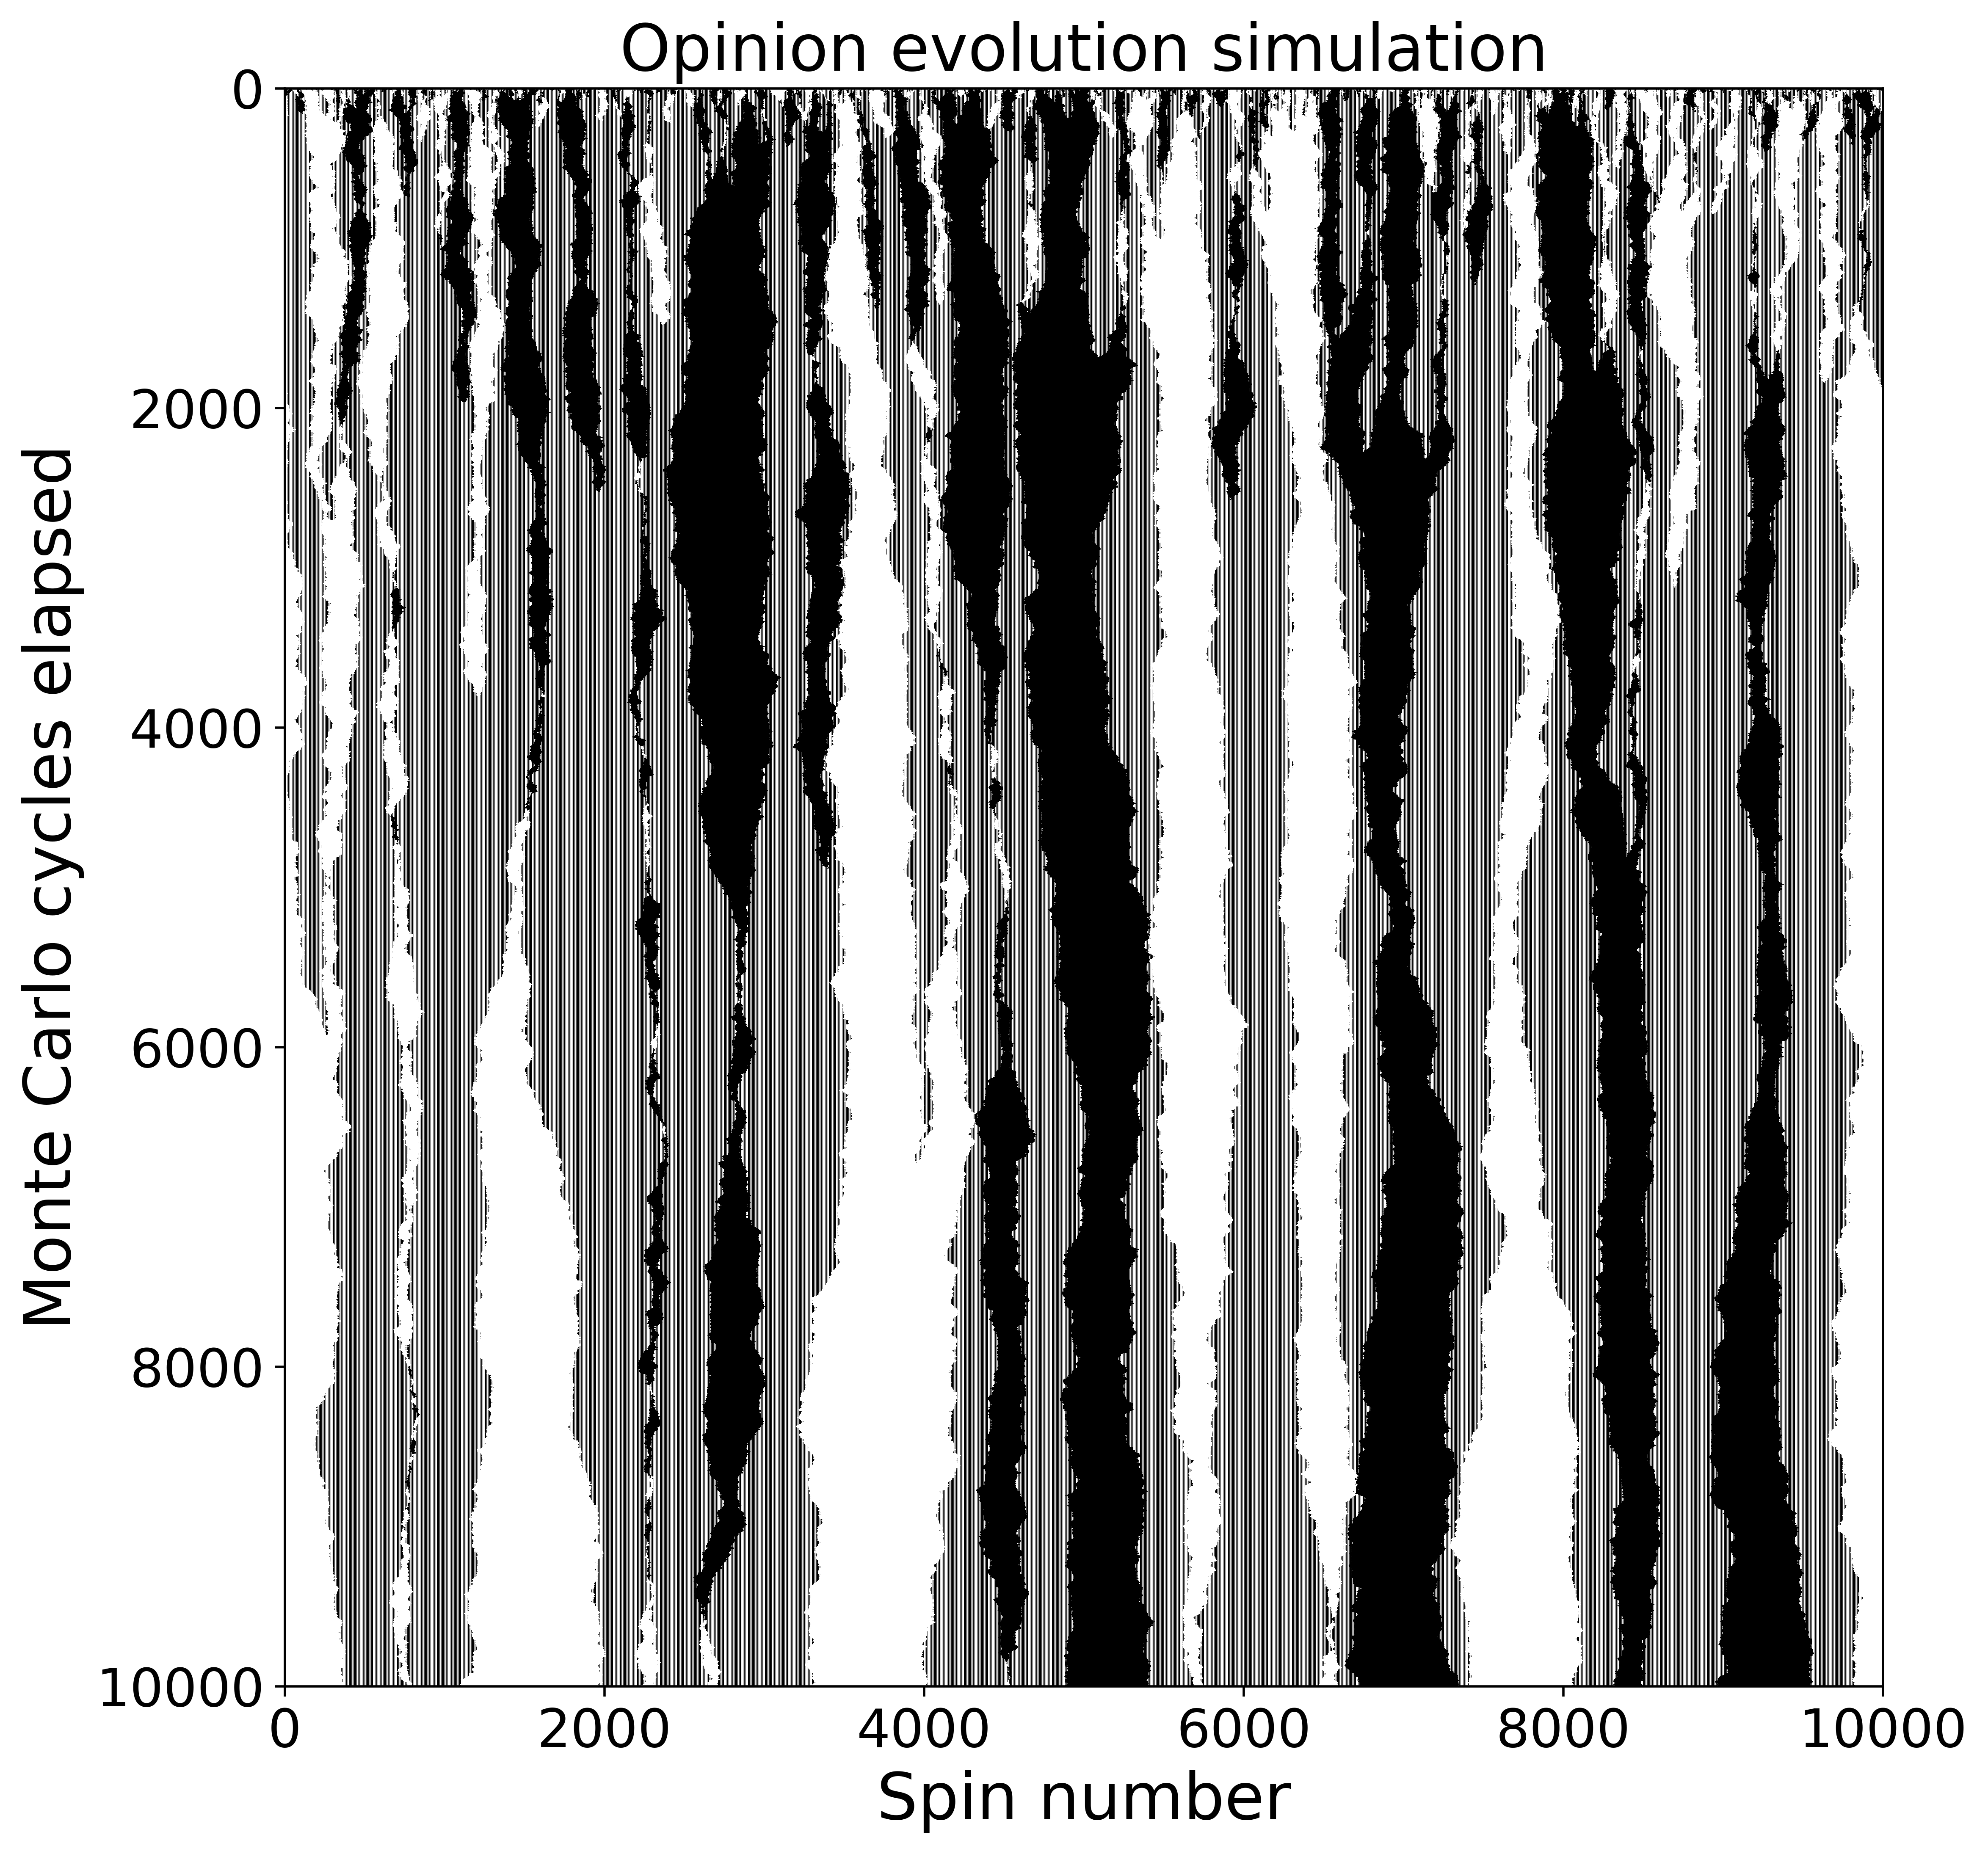
\includegraphics[width=0.8\textwidth]{periodic1.png}}
\caption{A realization with $10^4$ spins over $10^4$ MC-cycles with periodic boundary conditions.}
\label{fig:per}
\end{figure}

We ran an experiment with $10^5$ spins over $10^7$ MC-cycles. In Figure \ref{fig:menc} we see results from the realisations. The system is to large to plot as a time-evolution in the manner we have done throughout. Instead we have plotted the cluster size distribution, with the mean cluster size plotted over. As can be seen from the distributions the clusters vary in size at every stored step, with seemingly random fluctuations, but the mean cluster size evolves in steps, and it only increases. As the mean cluster size simply is the system size divided by the number of clusters, it is clear that the abrupt jumps in the plot represent the elimination of one or more clusters. At the end there are only 4 clusters remaining. Here we only have data points for every $10^4$ MC-cycle, but in a similar plot detailing the first 1000 MC-cycles (not included here) we saw that in the beginning clusters also can form, as we have discussed earlier, in the boundaries between decided clusters, such formation becomes impossible at a later stage.

\begin{figure}[H]
\centerline{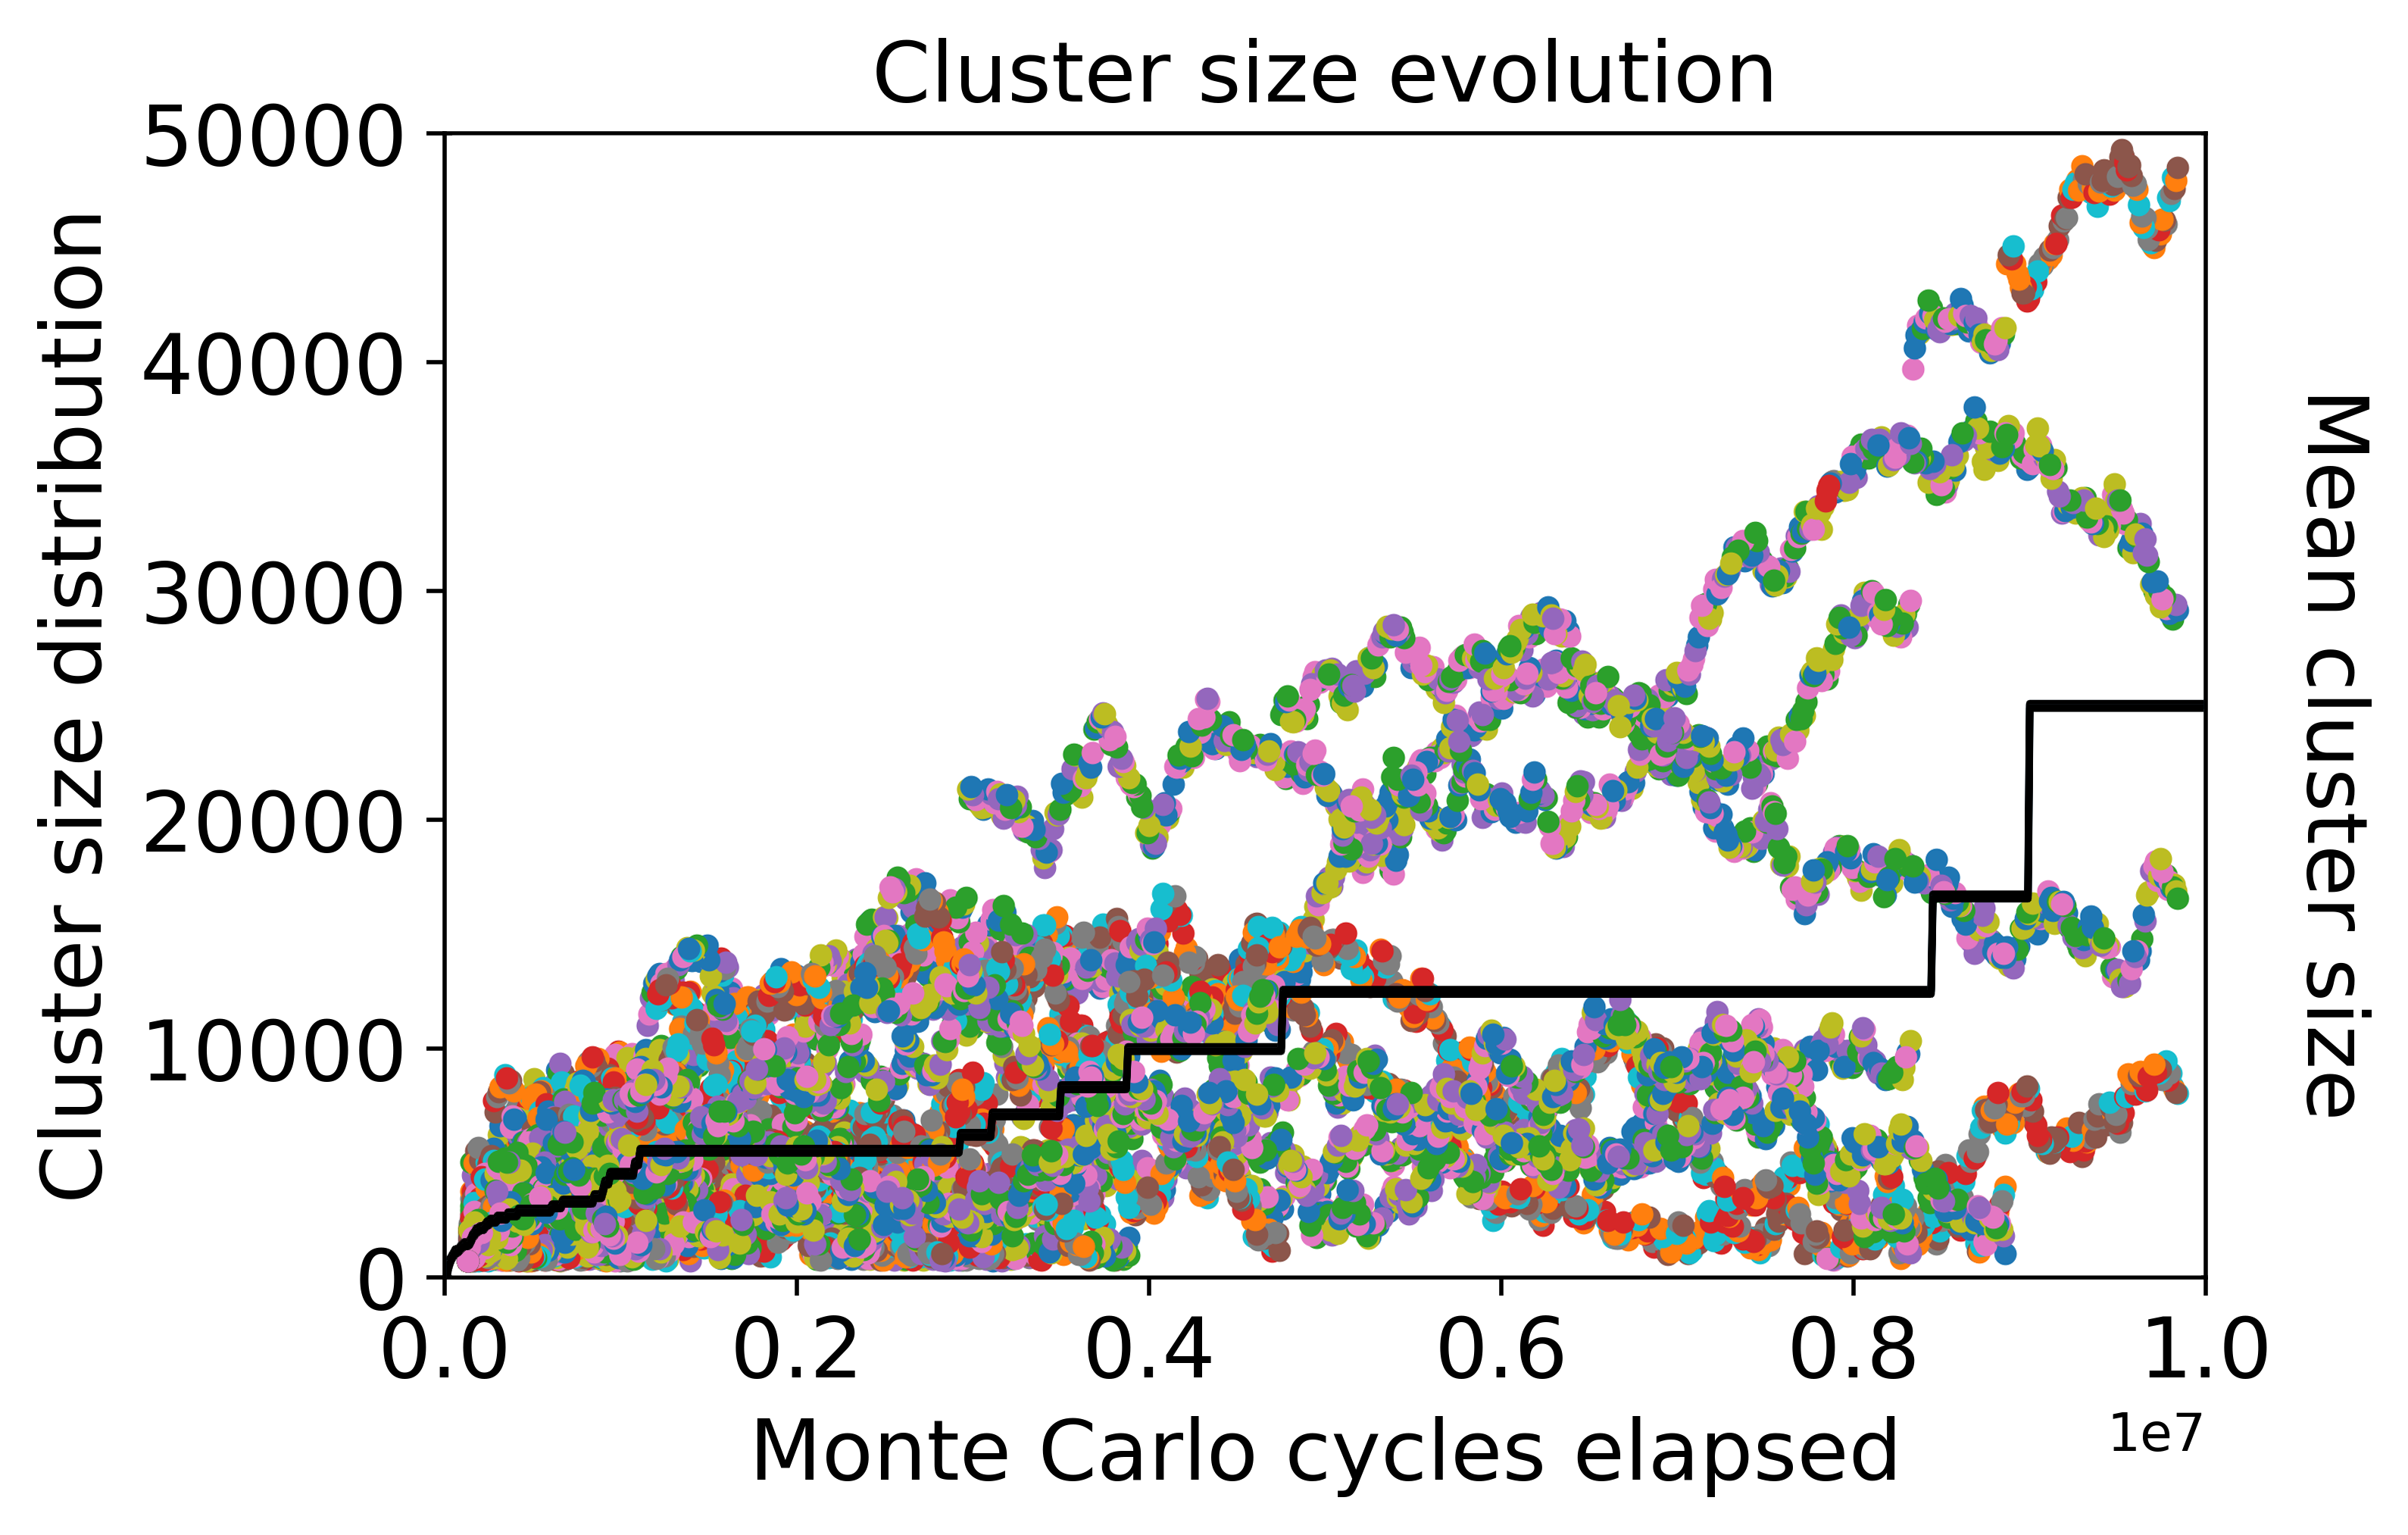
\includegraphics[width=0.8\textwidth]{meanCluster.png}}
\caption{Results for  $10^5$ spins over $10^7$ MC-cycles with periodic boundary conditions. The dots represent the cluster size distribution and the black line is the mean cluster size.}
\label{fig:menc}
\end{figure}

Clearly a system with $10^5$ spins is not infinite. With a truly infinite system, coupled with a truly random initialization and MC-draws, the evolution of the mean cluster sized should follow some well defined curve, with a very steep gradient through the initial steps, that quite early flattens out, as the well defined cluster configuration takes over.

\section{Conclusion}
We have implemented MC-simulations on 1D vectors with modified Ising rules to simulate opinion evolution in a closed community. By and large we confirm the findings of Katarzyna Sznajd-Weron and Józef Sznajd \cite{opinion}. We find the proposed model to be an interesting approach to understand opinion dynamics, but we also clearly feel that the model is somewhat arbitrary in terms of relating it to actual human communities. The full range of possible dynamics and outcomes by the model is overly simplistic, as only two opinions are allowed, and only the borders between clusters allow for dynamics. The introduction of noise in the model modifies this last condition, but in an overly random manner, this disrupting the physical nature imposed by the rules in the first place. The findings inspire the desire for further probing, for instance by implementation in 2D and 3D, or through modification or elaboration of the rules. It should also be noted that part of what truly makes the traditional Ising model relevant for modeling actual physical systems, is the coupling with the Boltzmann-distribution of mean energy as a function of temperature, which contribute vastly to the models sophistication and relevance. Such a coupling is not present in the model presented in this project, the system is not in any way tuned by any time dependent external variable, such an implementation could perhaps breathe more life into the simulations. These topics are more extensively discussed amongst others by Serge Galam \cite{galam}.

%\bibliographystyle{plain}
%\bibliographystyle{siam}
\bibliography{sample}
\bibliographystyle{IEEEtran}

\begin{appendix}




\end{appendix}
\end{document}
